% !TEX program = xelatex
\documentclass[12pt,a4paper]{article}


\usepackage{geometry}
\geometry{a4paper,left=2.5cm,right=2.5cm,top=2.5cm,bottom=2.5cm}
\usepackage{ctex}
\usepackage{sectsty}
\sectionfont{\centering}
\renewcommand\thesection{\chinese{section}、}
\renewcommand\thesubsection{\arabic{section}.\arabic{subsection}}
\usepackage[dvipsnames]{xcolor}
\usepackage{booktabs}
\usepackage{makecell}
\usepackage{amsfonts,amsmath,amssymb,mathtools}
\usepackage{multirow}
\usepackage{graphicx}
\usepackage{subcaption}
\usepackage{float}
\usepackage{enumitem}
\usepackage{array}
\usepackage{longtable}
\usepackage{listings}
\usepackage{fancyhdr}
\usepackage{hyperref}
\usepackage{url}
\usepackage{tabularx}
\usepackage{xltabular}

\hypersetup{
  colorlinks=true,
  linkcolor=black,
  urlcolor=blue,
  citecolor=black,
  pdfstartview=Fit,
  breaklinks=true
}

\lstset{
  frame=tb,
  aboveskip=3mm,
  belowskip=3mm,
  showstringspaces=false,
  columns=flexible,
  framerule=1pt,
  rulecolor=\color{gray!35},
  backgroundcolor=\color{gray!5},
  basicstyle={\small\ttfamily},
  numbers=left,
  numberstyle=\tiny\color{gray},
  keywordstyle=\color{blue},
  commentstyle=\color{ForestGreen},
  breaklines=true,
  breakatwhitespace=true,
  tabsize=3
}
\renewcommand{\lstlistingname}{源程序}

\newcommand{\tip}[1]{\par\noindent\textbf{【提示】} #1\par}
\newcommand{\warning}[1]{\par\noindent\textbf{【高频失分点】} #1\par}
\newcommand{\good}[1]{\par\noindent\textbf{【推荐写法】} #1\par}
\newcommand{\bad}[1]{\par\noindent\textbf{【不推荐写法】} #1\par}
\newcommand{\core}[1]{\boxed{\text{#1}}}

\fancyhf{}
\cfoot{\thepage}
\renewcommand{\headrulewidth}{0pt}
\pagestyle{fancy}


\usepackage[font=small,labelsep=quad]{caption}

\newcommand{\prompt}[1]{\par\noindent\textbf{【写作提示】}#1\par}      % 本节该写什么
\newcommand{\material}[1]{\par\noindent\textbf{【可用素材】}#1\par}    % 已有的数据/结论清单
\newcommand{\pitfall}[1]{\par\noindent\textbf{【容易失分】}#1\par}     % 常见问题
\newcommand{\ph}[1]{\textbf{【#1】}}                                   % 行内占位符
\newcommand{\figph}[1]{%
  \begin{center}
  \fbox{\parbox{0.72\textwidth}{\centering\vspace{2ex}#1\vspace{2ex}}}
  \end{center}}

\newcommand{\handbook}[2]{\par\noindent\textbf{【手册索引：#1】} #2\par}
\renewcommand{\boxed}[1]{#1}
\begin{document}
\linespread{1.05}\selectfont


\pagenumbering{arabic}
\setcounter{page}{1}

\begin{center}
{\zihao{-2}\bfseries 基于一维轴对称传热传质模型的药材烘干过程建模与仿真验证}


\vspace{2ex}
{\zihao{3}\bfseries 摘\quad 要}
\end{center}

\noindent 本文针对圆柱形中药材在变温变湿环境下的烘干问题，建立一维轴对称
传热--传质双向耦合模型，采用守恒型有限体积法自主求解，并以 COMSOL 有限元
仿真与积分守恒恒等式对结果作交叉验证，依次回答了预热平衡、全程干燥、
达标时长与考虑尺寸收缩的达标时长四个问题。

针对问题一，根据药材长径比达 6.25、端面面积仅占侧表面 $8\%$ 的几何特征，
忽略端面散热与轴向温度梯度，将圆柱药材抽象为半径方向的一维轴对称问题：
以傅里叶导热与菲克扩散分别描述热量与水分迁移，表面取第三类对流边界，
轴心取零通量对称条件，并把附件1 的离散环境数据插值为连续边界函数使模型
闭合；数值上采用守恒型有限体积法离散、全隐式时间推进、追赶法求解三对角
方程组。部分求解结果：1800~s 时中心温度 $33.5811^\circ\mathrm{C}$、表面
温度 $36.7842^\circ\mathrm{C}$，表面含水率降至 1.5145~kg/kg，而中心仍
保持初始值 2.5500~kg/kg，呈``热快质慢''的典型特征。

针对问题二，在问题一模型基础上把常数物性升级为随含水率变化的物性
（附录3），使传热与传质由解耦变为双向耦合：温度经 $D(C,T)$ 影响水分扩散
速率，水分经 $\rho(C)$、$c_p(C)$、$k(C)$ 影响温度演化，每一时间步用上一
时刻状态更新物性并迭代推进；针对附件1 仅覆盖前 4~h 的限制，对恒温干燥段
作常数外推以支撑 3~h 计算。部分求解结果：3~h 时中心温度
$49.8502^\circ\mathrm{C}$、中心含水率 1.7651~kg/kg、表面含水率
1.0084~kg/kg，径向温差缩小到 $0.12^\circ\mathrm{C}$。

针对问题三，将``各处水分均低于 0.15~kg/kg''转化为全域最大值判据：由抛物型
方程的极值原理，含水率最大值必在轴心取得，故只需追踪中心含水率，并把烘干
时长定义为该量首次低于 0.15~kg/kg 的时刻。部分求解结果：烘干时长 57.07~h
（约 2.38 天），与题目``$2\sim3$ 天''的先验判断一致。

针对问题四，附件2 给出的半径由 2.000~cm 单调收缩至 1.198~cm，计算域成为
移动区域。本文引入材料坐标变换把移动域固定为初始区间，并导出等效扩散放大
因子 $(R_0/R)^2$ 与表面传质项的半径修正，使收缩对干燥的加速作用进入方程；
同时用``忽略收缩''的对照计算说明收缩不可忽略。部分求解结果：考虑收缩时
烘干时长 50.75~h，比不考虑收缩缩短约 6.3~h（约 $11\%$）。

全文从三个层面检验结果可信度：用有限元与有限体积两种独立方法复算，问题一
至问题三全场相对偏差均小于 $1\%$、烘干时长偏差仅 $0.06\%$；网格加密一倍
误差减半（一阶收敛），Richardson 外推后与仿真值相差 $0.17\%$；与数值方法
无关的积分守恒恒等式检验残差小于 $2\%$ 且正负交替。灵敏度分析表明扩散系数
前置系数最敏感（$\pm20\%$ 扰动使烘干时长变化 $18.4\%$），传热系数几乎不
影响结果。模型可进一步推广至变径药材、二维轴对称几何以及以能耗与品质为
目标的烘干工艺优化。

\noindent\textbf{关键词：}传热传质耦合；一维轴对称；有限体积法；材料坐标变换；全域最大值判据；仿真验证

\clearpage

\section{问题重述}
\subsection{问题背景}
干燥是决定中药材成品品质的关键工序之一，热风烘干因其操作简便、适用范围广而成为常见的干燥方式。该过程主要包括预热平衡与恒温干燥两个阶段：通过调控烘房内的温度与水分浓度（湿度）环境，驱动热量由药材表面向内部传递、水分由内部向表面迁移并蒸发，从而协同完成药材脱水。

在实际烘干中，烘房温湿度、干燥时长等工艺参数选取不当，容易造成干燥效率偏低、能耗偏高以及药材内外含水率不均、成品品质不稳定等问题；而依靠反复试验摸索最优工艺的传统“试凑”模式又存在成本高、周期长的弊端。因此，亟需借助数理分析与数值仿真手段，刻画药材内部温度场与水分场的时空演化规律，为科学制定烘干工艺、提升干燥效率与成品质量提供依据。

\subsection{问题重述}
某中药材形状近似圆柱体，长 $25\ \mathrm{cm}$、半径 $2\ \mathrm{cm}$；烘干开始时药材整体温度为 $28\ \mathrm{^{\circ}C}$，水分浓度（即干基含水率）为 $2.55\ \mathrm{kg/kg}$；烘干过程中烘房的温度与水分浓度随时间变化（见附件1），各阶段所需的物性参数与经验公式分别由附录2—附录4给出，计算结果按指定格式填入附件3提供的 \texttt{result1—result4.xlsx} 模板，结果均保留四位小数。需由理想情形逐步逼近实际情形，依次解决以下四个问题。

\subsubsection{问题一：预热平衡阶段、定物性参数下的温度与水分浓度建模}
仅考虑预热平衡阶段，依据附录2给定的密度、比热容、热传导系数、对流换热系数、对流传质系数以及水分浓度扩散系数经验公式，建立描述药材内部温度和水分浓度随时间、随到中心距离变化规律的数学模型。要求按表1、表2给出 100, 300, 600, 900, 1200, 1500, 1800 $\mathrm{s}$ 时，距药材中心 $0, 0.5, 1, 1.5, 2\ \mathrm{cm}$ 处的温度与水分浓度，并将 $1800\ \mathrm{s}$ 内每隔 $1\ \mathrm{s}$、径向每隔 $0.1\ \mathrm{cm}$ 的完整结果保存至 \texttt{result1.xlsx}。

\subsubsection{问题二：覆盖全过程、物性参数随状态变化的温度与水分浓度建模}
实际烘干一般持续 $2\sim3$ 天，预热平衡与恒温干燥两阶段参数不同。为简化计算，统一采用附录3给出的经验公式（密度、比热容、热传导系数及水分扩散系数均随局部水分浓度 $C$ 和温度 $T$ 变化），建立贯穿整个烘干过程的温度场与水分浓度场模型。要求按表3、表4给出 $3\ \mathrm{h}$ 内每隔 $0.5\ \mathrm{h}$、距中心 $0, 0.5, 1, 1.5, 2\ \mathrm{cm}$ 处的结果，并将每隔 $1\ \mathrm{s}$、径向每隔 $0.1\ \mathrm{cm}$ 的完整结果保存至 \texttt{result2.xlsx}。

\subsubsection{问题三：满足含水率达标要求的烘干时长确定}
在问题二模型的基础上，以“药材各处水分浓度均低于 $0.15\ \mathrm{kg/kg}$”作为烘干达标（干燥终点）判据，确定药材烘干所需要的时间（单位：$\mathrm{h}$）。要求按表5给出每隔 $6\ \mathrm{h}$、径向每隔 $0.5\ \mathrm{cm}$ 的水分浓度（直至烘干结束时刻），并将每隔 $60\ \mathrm{s}$、径向每隔 $0.1\ \mathrm{cm}$ 的完整水分浓度结果保存至 \texttt{result3.xlsx}。

\subsubsection{问题四：考虑失水尺寸收缩的烘干时长确定}
实际烘干过程中，药材会随水分流失而发生尺寸（半径）收缩。结合附件2给出的药材半径随时间变化关系、采用附录4的经验公式，建立考虑尺寸变化（移动边界）的干燥模型，重新确定药材的烘干时长。要求按表6给出每隔 $6\ \mathrm{h}$、径向每隔 $0.5\ \mathrm{cm}$（直至药材表面）的水分浓度，并将每隔 $60\ \mathrm{s}$、径向每隔 $0.1\ \mathrm{cm}$ 的完整结果保存至 \texttt{result4.xlsx}。


\section{问题分析}
\subsection{问题一的分析}
针对问题一，已知药材为规则圆柱，圆柱的长径比为6.25，圆柱端面面积与侧面面积之比为$2\pi R^2/(2\pi RL)=R/L=2/25=8\%$，故可忽略端面效应，将问题抽象成一维圆柱径向非稳态传热与水分扩散问题。在此过程中，首先，已知的离散环境数据与传热传质方程所需的连续时间边界函数不符，必须把离散数据转化为连续边界条件，否则模型不闭合；其次，水分扩散系数依赖未知的含水率，使得水分方程为非线性方程，需要迭代处理；然后，圆柱坐标下扩散算子中含有$1/r$因子，在轴心发散，离散需做对称性处理。进一步作量级估计，热扩散与水分扩散的特征时间分别约为 40 min 与 22 h，表明药材内部径向梯度不可忽略、须采用分布参数模型，且预热阶段以升温为主、干燥尚未充分展开。据此，将问题化归为一维轴对称的抛物型初边值问题：内部采用傅里叶导热与菲克扩散描述热量与水分传递，表面采用对流换热与对流传质的第三类边界条件，轴心采用零通量的对称条件，初始为均匀场，并用守恒型格式离散；其中题目未给出的汽化潜热等参数不显式计入。这一模型及其离散框架将作为后三问的共同基础。

\subsection{问题二的分析}
针对问题二，在问题一建立的一维径向非稳态传热与水分扩散模型的基础上，本问进一步要求刻画药材在整个烘干过程中的温湿演化。本问与问题一的差异，并不在于几何或控制方程结构的改变，而在于以下两点：一是物性由常数升级为状态变量的函数，二是时间尺度由30分钟扩展到2--3天。因此，物性的函数化使传热方程与水分方程由解耦变为双向耦合——温度经 $D(C,T)$ 影响水分扩散速率，水分经 $\rho(C)$、$c_p(C)$、$k(C)$ 影响温度演化，两条方程须联立求解；相应地，每个时间步的离散系统由线性变为非线性，需迭代更新物性，而守恒离散与全隐式推进的框架仍沿用问题一。针对时间尺度的延长，我们对恒温干燥阶段的边界条件进行补足：附件 1 仅覆盖前 4 h，故取附件 1 末值作常数外推（$T_\infty\rightarrow50.16\ ^\circ\text{C}$、$C_\infty\rightarrow0.0499\ \text{kg/kg}$）。本问的初始条件与边界条件形式不变，仅需补充上述外推规则；同时本问仍为机理正问题，不涉及优化目标。

\subsection{问题三的分析}
针对问题三，本问要求在问题二所建立的全程干燥模型的基础上，确定药材上各点水分均低于$0.15\ \text{kg/kg}$所需的烘干时间。基于此，本问无需引入新的控制方程与物性，而是在问题二模型上增加一个“烘干达标”的终止判据。首先，若将“各点的水分均低于0.15”此条件数学化：记药材内部的最大含水率为 $M(t)=\max_{0\leq r\leq R} C(r,t)$，则问题转化为求 $M(t)<0.15$，烘干时长 $t^*$ 定义为该条件首次成立的时刻，即 $t^*=\min\{t>0: M(t)<0.15\}$。其次，药材表面是对流传质出流边界、轴心是零通量对称面，水分始终由中心向表面单向扩散，含水率沿径向单调递减，因此中心最湿、表面最干，最大含水率在中心取得，即 $M(t)=C(0,t)$；这一结论亦由抛物型方程的极值原理严格保证：含水率的空间最大值只能出现在边界上，而表面为出流边界、含水率向表面递减，故该最大值必在轴心。然后，在干燥过程中， $C(0,t)$ 关于时间单调递减，$f(t)=C(0,t)-0.15$ 为单调函数，求 $t^*$ 等价于求该函数的唯一零点；该零点可用时步扫描或二分法求解，其精度由时间步长与网格的收敛性检验保证。

\subsection{问题四的分析}
针对问题四，本问相对于问题三的新增要素在于几何本身随着时间变化：附件2中给出的半径由 2.0 cm 单调收缩至约 1.198 cm，这意味着计算域 $[0,R(t)]$ 是一个移动区域。因此，问题三中的控制方程、边界条件与网格都必须随几何变化而修正，其中表面边界通量中的半径须改用当前半径 $R(t)$，而非初始半径。基于此，为了处理移动边界，本文采用跟随材料收缩的材料坐标（拉格朗日坐标）来固定计算域：记材料点的初始位置为 $X\in[0,R_0]$，其当前物理位置满足 $r=X\cdot R(t)/R_0$，从而将方程变换到固定的材料区间 $[0,R_0]$ 上求解。但同时，方程中出现与 $R(t)$ 有关的缩放因子——扩散项放大 $(R_0/R)^2$ 倍、表面通量放大 $R_0^2/R$ 倍，物理上对应“扩散路程变短、单位干物质表面积增大”，均使干燥加快。另外，还需明确坐标约定：表 6 与 result4.xlsx 中“到药材中心的距离”指当前实际径向位置，末列“药材表面”为当前半径 $R(t)$，它与材料坐标经 $r=X\cdot R(t)/R_0$ 换算，以免表 6 因收缩而被误读。此外，为验证尺寸收缩的必要性，本文设置“忽略收缩”的对照计算，对比表明：忽略收缩时药材在给定烘干时长内无法达标，说明尺寸变化是问题四中不可忽略的决定性因素。


\section{模型假设}
根据题干和附录，本题的建模假设及其理由与影响列于表 \ref{tab:assumptions}。
\begin{xltabular}{\textwidth}{@{}c@{\hspace{3em}}>{\raggedright\arraybackslash}p{4.2cm}@{\hspace{1.8em}}>{\raggedright\arraybackslash}X@{}}
  \caption{模型假设及其理由}
  \label{tab:assumptions} \\
  \hline
  序号 & 假设 & 理由 \\
  \hline
  \endfirsthead

  \multicolumn{3}{c}{\small 续表} \\
  \hline
  序号 & 假设 & 理由 \\
  \hline
  \endhead

  \hline
  \multicolumn{3}{r}{\small 续下页} \\
  \endfoot

  \hline
  \endlastfoot

  H1 & 药材内部各向同性、连续介质，局部热平衡
     & 药材尺寸小且导热快，热扩散时间 $\tau_T \sim R^2/\alpha \approx 39\ \mathrm{min}$，热平衡时间远小于烘干时间。 \\
  \hline
  H2 & 水分迁移服从 Fick 扩散定律，扩散系数 $D$ 按照题干的经验公式
     & 题干中 $D$ 的经验公式已经指定用宏观 Fick 扩散描述水分迁移，无需考虑其他复杂驱动。 \\
  \hline
  H3 & 热量传递由导热控制，表面对流按牛顿冷却定律
     & 附录2中给出了 $h$，正文中使用第三类边界条件。由于毕渥数 $Bi \approx 1.39$，应使用内部导热结合表面对流的第三类边界条件。 \\
  \hline
  H4 & 模型按一维轴对称搭建
     & 端面占比约为 $7.4\%$，在模型假设的范围之内。 \\
  \hline
  H5 & 问题 1$\sim$3 药材几何尺寸不变
     & 题干中只有问题 4 给出半径变化数据，因此问题 1$\sim$3 按固定尺寸处理。 \\
  \hline
  H6 & 水分仅通过药材外表面与烘房空气对流传质交换，轴心 $r=0$ 处为对称面且无水分通量
     & 圆柱轴对称且 $Bi_{m} \approx 3.24$，表面与内部传质阻力相当，需用对流传质边界。 \\
  \hline
  H7 & 物性只依赖当前含水率（和温度），与历史无关
     & 题干经验公式规定了“当前状态决定物性”。 \\
  \hline
  H8 & 问题 4 中收缩为均匀收缩，即材料点到轴心的相对位置不变
     & 便于数值求解、便于与文献中的干燥收缩模型对照，且与一维变形域平滑方程的解一致。 \\
  \hline
  
\end{xltabular}


\subsection*{关键假设影响分析:}

\begin{enumerate}
       \item 针对假设H3，由于问题给定了对流换热系数h，且完全没有提供辐射换热与蒸发潜热的相关参数，因此忽略辐射换热与蒸发潜热、只考虑导热和对流是合理的简化。若放宽此假设将辐射换热和蒸发潜热考虑在内，通过近似参数推测，会对结果产生$10\% \sim 20\%$的影响。
       \item 针对假设H4，若放宽一维轴对称假设，考虑二维或三维模型，将会大大增加计算复杂度，但由于端面占比仅为7.4\%，对结果的影响量级预计在5\%以内。
\end{enumerate}


\section{符号说明}


本文主要符号按其在正文中出现的先后顺序说明如下，单位均采用国际单位制（SI）。
\begin{longtable}{>{\centering\arraybackslash}p{3cm}
                  >{\centering\arraybackslash}p{8cm}
                  >{\centering\arraybackslash}p{2cm}}
\caption{主要符号说明}
\label{tab:symbols}\\
\toprule
符号 & 说明 & 单位\\
\midrule
\endfirsthead

\toprule
符号 & 说明 & 单位\\
\midrule
\endhead

\bottomrule
\endlastfoot

$R$         & 药材半径 & m \\
$L$         & 药材长度 & m \\
$r$         & 径向坐标（到药材中心的距离） & m \\
$t$         & 时间 & s \\
$T$         & 药材温度 & $^\circ$C \\
$C$         & 干基含水率（水分浓度） & kg/kg \\
$\rho$      & 药材密度 & kg/m$^3$ \\
$c_p$       & 定压比热容 & J/(kg$\cdot$K) \\
$k$         & 导热系数 & W/(m$\cdot$K) \\
$h$         & 对流换热系数 & W/(m$^2\cdot$K) \\
$h_m$       & 对流传质系数 & m/s \\
$D$         & 水分扩散系数 & m$^2$/s \\
$T_\infty$  & 烘房空气温度 & $^\circ$C \\
$C_\infty$  & 烘房空气水分浓度 & kg/kg \\
$\alpha$    & 热扩散系数 & m$^2$/s \\
$M(t)$      & 全场最大含水率 & kg/kg \\
$t_{\mathrm d}$     & 烘干时长 & h \\
$f(t)$      & 判据函数，$f(t)=C(0,t)-0.15$ & kg/kg \\
$R(t)$      & 随时间变化的药材半径 & m \\
$R_0$       & 药材初始半径 & m \\
$X$         & 材料坐标（质点的初始径向位置） & m \\
$\tau$      & 特征时间 & s \\
$Bi$        & 毕渥数 & 无量纲 \\

\end{longtable}
注：$D$ 的经验公式中温度须取开尔文温标，即 $T_{\mathrm{K}}=T/^\circ\mathrm{C}+273.15$；
$\rho$、$c_p$、$k$、$D$ 在问题二、三、四中为对应经验式给出的变物性。


\section{模型的建立与求解}


\subsection{问题一模型的建立与求解}

\subsubsection{一维轴对称传热传质模型的建立}

将药材近似为半径 $R=0.02\ \mathrm{m}$、长度 $L=0.25\ \mathrm{m}$ 的均匀圆柱体。
题目中的“到药材中心距离”解释为圆柱中截面上到中心轴线的径向距离。药材长径比为
\begin{equation}
\frac{L}{2R}=6.25.
\end{equation}
\begin{equation}
\alpha=\frac{k}{\rho c_p}
=\frac{0.36}{820\times2600}
=1.6886\times10^{-7}\ \mathrm{m^2/s}.
\end{equation}
当 $t=1800\ \mathrm{s}$ 时，热扩散特征长度为
\begin{equation}
\ell_T=\sqrt{\alpha t}\approx1.743\ \mathrm{cm}.
\end{equation}

水分扩散系数随水分浓度变化。由于
\begin{equation}
\frac{\mathrm{d}D}{\mathrm{d}C}
=
D(C)\frac{0.89}{C^2}>0,
\end{equation}
故问题一阶段的最大水分扩散系数出现在初始水分浓度
$C_0=2.55\ \mathrm{kg/kg}$ 处，即
\begin{equation}
D_{\max}
=
7\times10^{-9}
\exp\left(-\frac{0.89}{2.55}\right)
=
4.9377\times10^{-9}\ \mathrm{m^2/s}.
\end{equation}
当 $t=1800\ \mathrm{s}$ 时，水分扩散特征长度为
\begin{equation}
\ell_C=\sqrt{D_{\max}t}\approx0.298\ \mathrm{cm}.
\end{equation}

由于 $\ell_T$ 和 $\ell_C$ 均远小于圆柱半长
$L/2=12.5\ \mathrm{cm}$，两个端面对圆柱中截面的影响可以忽略。
因此，本文忽略轴向和周向梯度，将有限长圆柱中截面的传热传质过程
简化为
\begin{equation}
0\le r\le R
\end{equation}
上的\textbf{一维轴对称径向问题}。

设 $T(r,t)$ 为药材内部温度，$C(r,t)$ 为药材干基水分浓度，
$T_a(t)$ 和 $C_a(t)$ 分别为烘房温度和烘房水分浓度。

\subsubsection{烘房时变边界函数}

附件1给出了离散时刻的烘房温度和水分浓度，而连续数学模型需要
任意时刻的环境边界值。为此，本文采用分段线性插值构造
$T_a(t)$ 和 $C_a(t)$，即相邻两个实测点之间用一条直线近似，整个区间由一串首尾相连的直线段组成。对于 $t_i\le t\le t_{i+1}$，有
\begin{equation}
T_a(t)
=
T_{a,i}
+
\frac{T_{a,i+1}-T_{a,i}}{t_{i+1}-t_i}
(t-t_i),
\end{equation}
\begin{equation}
C_a(t)
=
C_{a,i}
+
\frac{C_{a,i+1}-C_{a,i}}{t_{i+1}-t_i}
(t-t_i).
\end{equation}

分段线性插值不会在相邻观测点之间引入额外的极值点。而高阶插值由于多项式振荡，容易产生非物理的过冲现象，导致插值结果出现数据中原本不存在的极大或极小值。后续数学模型求解和COMSOL验证均使用相同的边界函数，以保证比较条件一致。

\subsubsection{温度场控制方程}

根据能量守恒定律，药材内部单位体积的能量积累等于净导热流入
由Fourier热传导定律
\begin{equation}
q_T=-k\frac{\partial T}{\partial r},
\end{equation}
可得一维圆柱坐标下的非稳态热传导方程
\begin{equation}
\boxed{
\rho c_p\frac{\partial T}{\partial t}
=
\frac{1}{r}
\frac{\partial}{\partial r}
\left(
kr\frac{\partial T}{\partial r}
\right)
},
\qquad
0<r<R,\quad 0<t\le1800.
\label{eq:q1-heat}
\end{equation}

由于问题一中的 $\rho$、$c_p$ 和 $k$ 均为常数，式
\eqref{eq:q1-heat}也可以写为
\begin{equation}
\frac{\partial T}{\partial t}
=
\alpha
\left(
\frac{\partial^2T}{\partial r^2}
+
\frac{1}{r}\frac{\partial T}{\partial r}
\right),
\qquad
\alpha=\frac{k}{\rho c_p}.
\end{equation}

此处由于题目未给出汽化潜热、干物质密度和蒸发区域等参数，我们设定假设H3，即不显式考虑水分蒸发对温度场的潜热反馈，以避免引入不可辨识参数。

\subsubsection{水分浓度场控制方程}

根据Fick扩散定律，药材内部径向水分通量为
\begin{equation}
J_C=-D(C)\frac{\partial C}{\partial r}.
\end{equation}
结合质量守恒关系，可得一维轴对称非线性水分扩散方程
\begin{equation}
\boxed{
\frac{\partial C}{\partial t}
=
\frac{1}{r}
\frac{\partial}{\partial r}
\left[
rD(C)\frac{\partial C}{\partial r}
\right]
},
\qquad
0<r<R,\quad 0<t\le1800.
\label{eq:q1-moisture}
\end{equation}

水分扩散系数采用题目给出的经验公式
\begin{equation}
\boxed{
D(C)
=
7\times10^{-9}
\exp\left(-\frac{0.89}{C}\right)
}.
\label{eq:q1-diffusivity}
\end{equation}

由于 $D$ 随未知量 $C$ 变化，式\eqref{eq:q1-moisture}为变系数
非线性抛物型偏微分方程。随着水分浓度降低，$D(C)$ 逐渐减小，
药材内部水分迁移阻力随之增大。

\subsubsection{初始条件与边界条件}

烘干开始时，药材内部温度和水分浓度均匀分布，因此初始条件为
\begin{equation}
\boxed{
T(r,0)=28,\qquad C(r,0)=2.55
},
\qquad 0\le r\le R.
\label{eq:q1-initial}
\end{equation}

在圆柱中心轴线 $r=0$ 处，由轴对称性可得零通量条件
\begin{equation}
\boxed{
\left.\frac{\partial T}{\partial r}\right|_{r=0}=0,
\qquad
\left.\frac{\partial C}{\partial r}\right|_{r=0}=0
}.
\label{eq:q1-center}
\end{equation}

在药材侧表面 $r=R$ 处，采用第三类边界条件。温度场满足
\begin{equation}
\boxed{
-k\left.\frac{\partial T}{\partial r}\right|_{r=R}
=
h_T\left[T(R,t)-T_a(t)\right]
},
\label{eq:q1-heat-bc}
\end{equation}
水分浓度场满足
\begin{equation}
\boxed{
-D(C)\left.\frac{\partial C}{\partial r}\right|_{r=R}
=
h_C\left[C(R,t)-C_a(t)\right]
}.
\label{eq:q1-moisture-bc}
\end{equation}

式\eqref{eq:q1-heat-bc}和式\eqref{eq:q1-moisture-bc}分别表示
药材内部传导通量、扩散通量与表面对流交换通量相平衡。

在问题一给定的参数体系中，温度控制方程不含水分浓度，
水分控制方程也不含温度，因此两个子模型不存在显式耦合，
可以分别进行数值求解。

\begin{figure}[H]
\centering
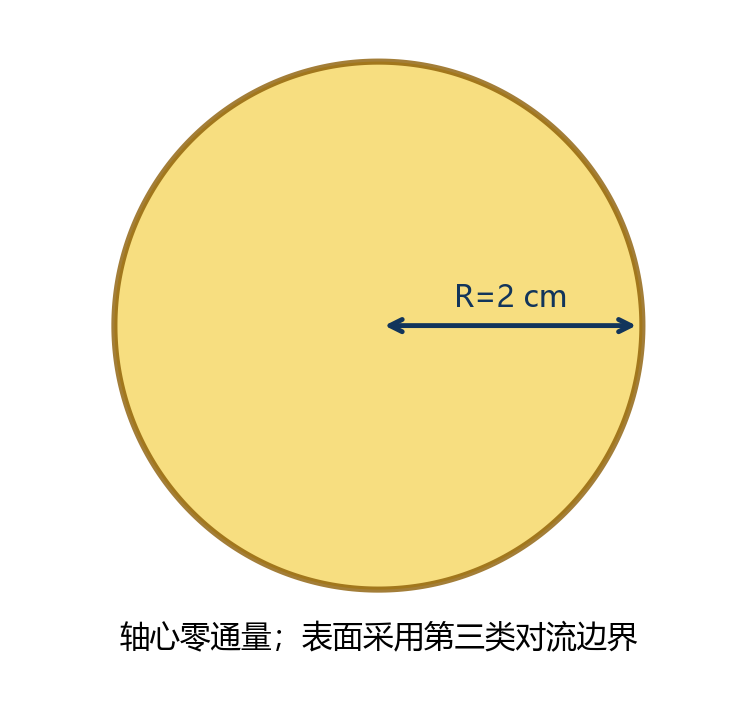
\includegraphics[width=0.70\textwidth]{image_tex/q1_schematic.png}
\caption{圆柱药材的几何模型与一维轴对称边界条件}
\label{fig:q1-schematic}
\end{figure}

\subsubsection{基于有限体积法的模型离散}

为了求解上述连续偏微分方程，本文采用一维轴对称有限体积法进行
空间离散，并采用全隐式格式推进时间。

需要强调的是，题目要求的 $0.1\ \mathrm{cm}$ 是结果输出间隔，
并不等同于内部计算网格。由于传质Biot数较大，药材表面附近可能
形成较陡的水分梯度，因此内部采用向 $r=R$ 加密的非均匀网格，
计算完成后再将结果抽取到题目指定位置。

设径向节点为
\begin{equation}
0=r_0<r_1<\cdots<r_N=R,
\end{equation}
节点 $r_i$ 所对应控制体的内、外表面分别为
$r_{i-\frac12}$ 和 $r_{i+\frac12}$。忽略公共因子后，
第 $i$ 个控制体的几何权重为
\begin{equation}
V_i=
\frac{1}{2}
\left(
r_{i+\frac12}^{2}-r_{i-\frac12}^{2}
\right).
\label{eq:q1-volume}
\end{equation}

采用全隐式时间格式，温度方程离散为
\begin{equation}
\begin{aligned}
\rho c_pV_i
\frac{T_i^{n+1}-T_i^n}{\Delta t}
={}&
kr_{i+\frac12}
\frac{T_{i+1}^{n+1}-T_i^{n+1}}
{r_{i+1}-r_i}\\
&-
kr_{i-\frac12}
\frac{T_i^{n+1}-T_{i-1}^{n+1}}
{r_i-r_{i-1}}.
\end{aligned}
\label{eq:q1-heat-fvm}
\end{equation}

水分浓度方程离散为
\begin{equation}
\begin{aligned}
V_i
\frac{C_i^{n+1}-C_i^n}{\Delta t}
={}&
r_{i+\frac12}D_{i+\frac12}^{n+1}
\frac{C_{i+1}^{n+1}-C_i^{n+1}}
{r_{i+1}-r_i}\\
&-
r_{i-\frac12}D_{i-\frac12}^{n+1}
\frac{C_i^{n+1}-C_{i-1}^{n+1}}
{r_i-r_{i-1}}.
\end{aligned}
\label{eq:q1-moisture-fvm}
\end{equation}

相邻控制体界面的扩散系数采用调和平均：
\begin{equation}
D_{i+\frac12}
=
\frac{2D_iD_{i+1}}{D_i+D_{i+1}}.
\label{eq:q1-harmonic}
\end{equation}
该处理能够保持相邻控制体之间的水分通量连续。

在中心轴线 $r=0$ 处，控制体内侧表面积为零，因此内侧通量自然
消失，无需直接计算连续方程中的 $1/r$，也无需设置虚拟节点。

在最外层控制体中，温度和水分的表面对流通量分别写为
\begin{equation}
Rh_T\left[T_a(t^{n+1})-T_N^{n+1}\right]
\end{equation}
和
\begin{equation}
Rh_C\left[C_a(t^{n+1})-C_N^{n+1}\right].
\end{equation}

\subsubsection{非线性迭代与方程组求解}

温度方程为常系数线性方程，每个时间步只需组装并求解一次
三对角线性方程组。

水分浓度方程中，$D=D(C)$ 与新时刻的未知水分浓度有关。
因此，在每一个时间步内采用Picard迭代处理非线性。以旧时刻
水分浓度作为初始迭代值：
\begin{equation}
C_i^{n+1,(0)}=C_i^n.
\end{equation}
第 $m$ 次迭代先计算
\begin{equation}
D_i^{(m)}
=
7\times10^{-9}
\exp\left(
-\frac{0.89}{C_i^{n+1,(m)}}
\right),
\end{equation}
再组装式\eqref{eq:q1-moisture-fvm}并求得
$C_i^{n+1,(m+1)}$。

当满足
\begin{equation}
\max_{0\le i\le N}
\left|
C_i^{n+1,(m+1)}
-
C_i^{n+1,(m)}
\right|
<\varepsilon
\label{eq:q1-picard-stop}
\end{equation}
时，认为当前时间步的非线性迭代收敛。

有限体积离散后，温度场和水分场均形成三对角线性方程组，
因此采用Thomas追赶法求解。该算法的时间复杂度为
$O(N)$
适合在大量时间步上重复计算。

\subsubsection{输出与数值精度控制}

内部计算时间步记为 $\Delta t_{\mathrm{in}}$，题目要求的结果
输出步长记为 $\Delta t_{\mathrm{out}}=1\ \mathrm{s}$。
二者相互独立，即
\begin{equation}
\Delta t_{\mathrm{in}}
\neq
\Delta t_{\mathrm{out}}.
\end{equation}
程序采用较小的内部时间步进行推进，仅在整数秒保存结果。

同理，内部采用表面加密的非均匀径向网格，模型计算完成后，
将数值解抽取到
\begin{equation}
r=0,0.001,\ldots,0.020\ \mathrm{m}
\end{equation}
的题目指定位置。

为控制离散误差，分别增加内部径向节点数并减小时间步，
比较中心、内部和表面位置的温度及水分浓度。当网格与时间步
进一步加密后，题目要求输出位置上的结果基本不再变化时，
认为数值解达到网格和时间步收敛。

\subsubsection{数学模型求解结果}

根据上述有限体积模型和数值算法，计算
$0\le t\le1800\ \mathrm{s}$、$0\le r\le0.02\ \mathrm{m}$
范围内的温度场和水分浓度场。

\begin{table}[H]
\centering
\caption{30 分钟内药材的温度（单位：$^\circ$C）}
\label{tab:t}
\begin{tabular}{cccccc}
\toprule
\multirow{2}{*}{时间/s}
& \multicolumn{5}{c}{到药材中心的距离/cm}\\
\cmidrule(lr){2-6}
& $0$ & $0.5$ & $1.0$ & $1.5$ & $2.0$\\
\midrule
$100$  & 28.0001 & 28.0004 & 28.0043 & 28.0333 & 28.1796\\
$300$  & 28.0416 & 28.0644 & 28.1525 & 28.3696 & 28.8474\\
$600$  & 28.4555 & 28.5382 & 28.8063 & 29.3186 & 30.1632\\
$900$  & 29.3277 & 29.4617 & 29.8790 & 30.6201 & 31.7283\\
$1200$ & 30.5471 & 30.7142 & 31.2270 & 32.1176 & 33.4256\\
$1500$ & 32.0010 & 32.1921 & 32.7715 & 33.7520 & 35.1186\\
$1800$ & 33.5811 & 33.7778 & 34.3702 & 35.3685 & 36.7842\\
\bottomrule
\end{tabular}
\end{table}

\begin{table}[H]
\centering
\caption{30 分钟内药材的水分浓度（单位：kg/kg）}
\label{tab:c}
\begin{tabular}{cccccc}
\toprule
\multirow{2}{*}{时间/s}
& \multicolumn{5}{c}{到药材中心的距离/cm}\\
\cmidrule(lr){2-6}
& $0$ & $0.5$ & $1.0$ & $1.5$ & $2.0$\\
\midrule
$100$  & 2.5500 & 2.5500 & 2.5500 & 2.5500 & 2.2557\\
$300$  & 2.5500 & 2.5500 & 2.5500 & 2.5492 & 2.0582\\
$600$  & 2.5500 & 2.5500 & 2.5500 & 2.5352 & 1.8832\\
$900$  & 2.5500 & 2.5500 & 2.5497 & 2.5043 & 1.7603\\
$1200$ & 2.5500 & 2.5500 & 2.5482 & 2.4642 & 1.6636\\
$1500$ & 2.5500 & 2.5499 & 2.5445 & 2.4202 & 1.5833\\
$1800$ & 2.5500 & 2.5497 & 2.5382 & 2.3749 & 1.5145\\
\bottomrule
\end{tabular}
\end{table}

\subsubsection{结果与分析}
\begin{figure}[H]
\centering
\begin{subfigure}{0.49\textwidth}
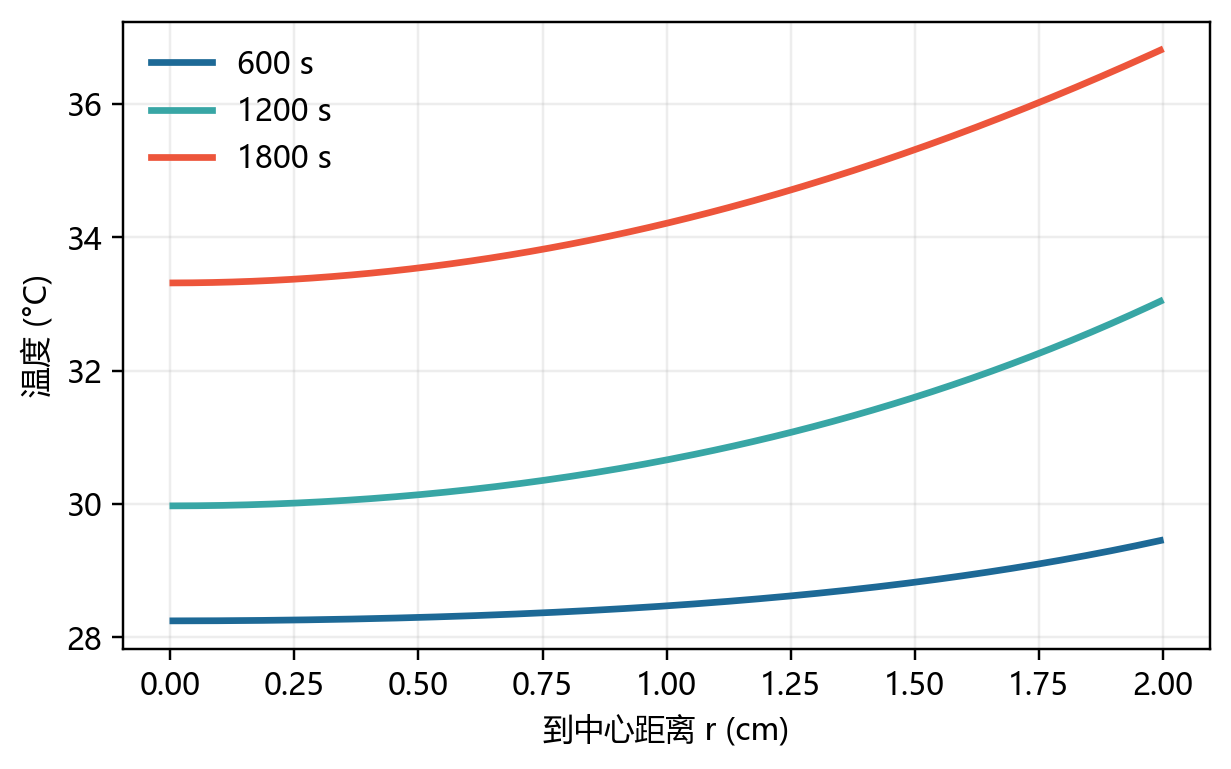
\includegraphics[width=\textwidth]{image_tex/q1_T_profile.png}
\caption{温度径向分布}
\end{subfigure}
\begin{subfigure}{0.49\textwidth}
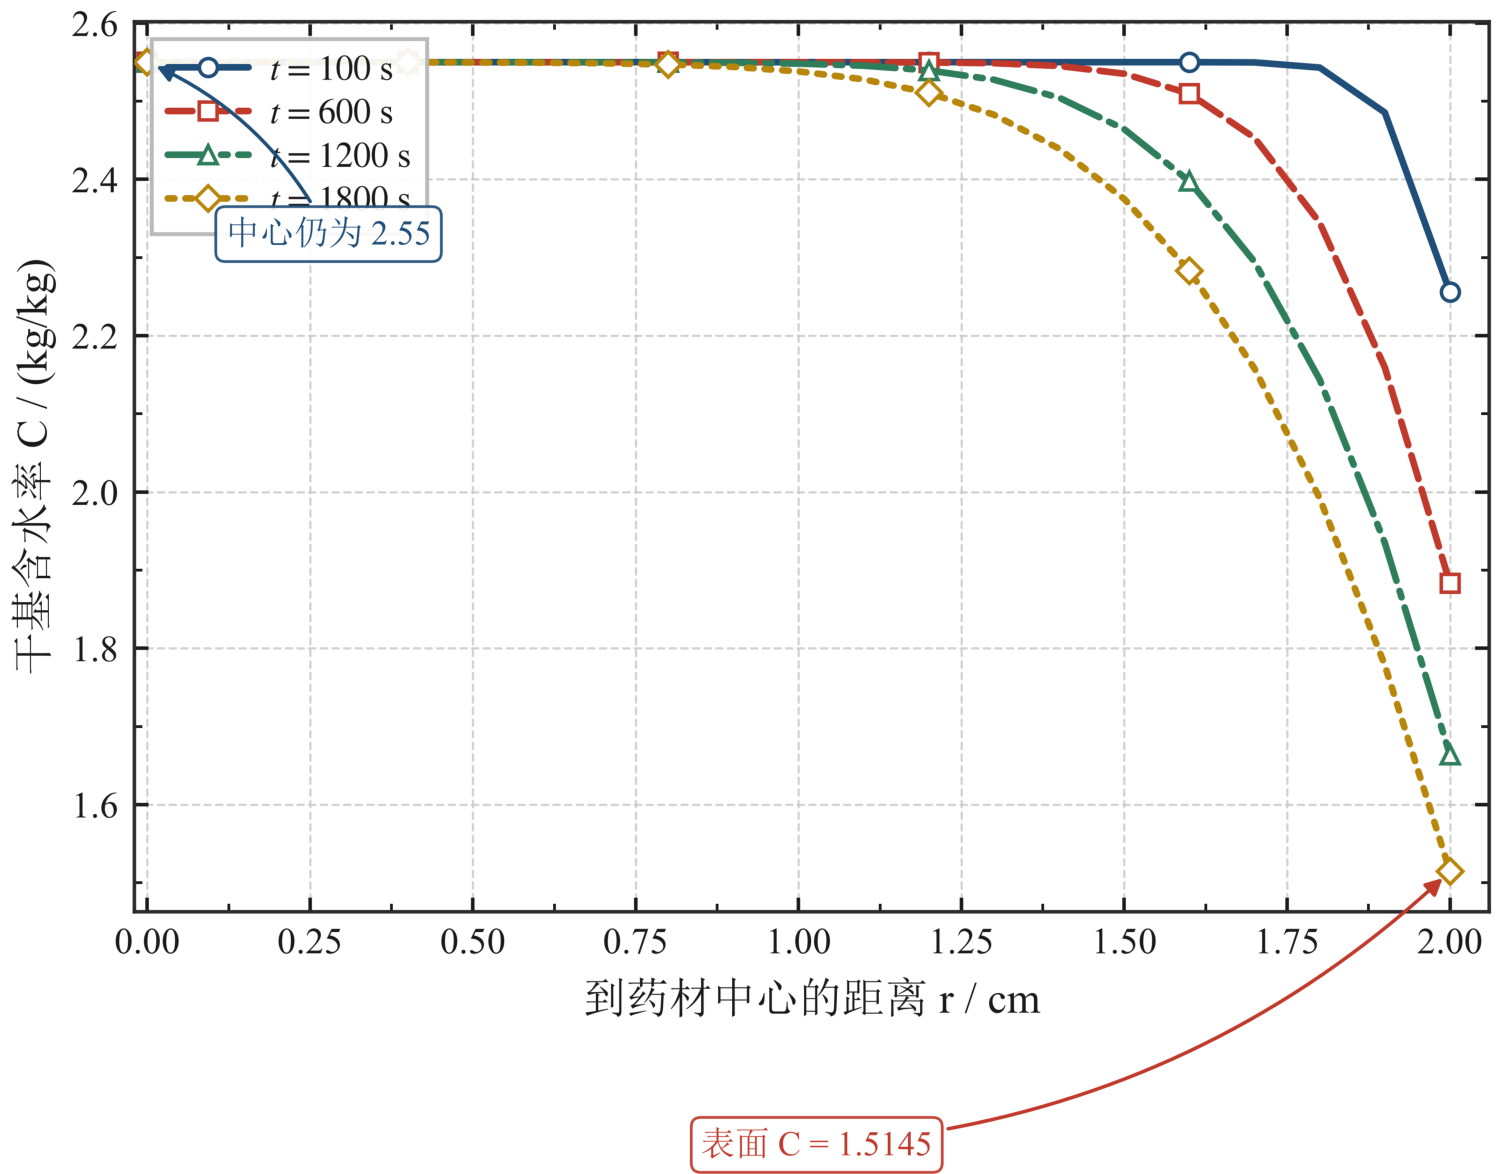
\includegraphics[width=\textwidth]{image_tex/q1_C_profile.png}
\caption{水分浓度径向分布}
\end{subfigure}
\caption{不同时刻药材内部温度与水分浓度的径向分布}
\label{fig:q1-profiles}
\end{figure}


根据上述数值模型与算法，得到预热阶段（0--1800~s）药材温度与含水率
随时间的演化，表~\ref{tab:t}、表~\ref{tab:c} 分别给出 7 个时刻、
5 个径向位置的结果。

温度场整体持续升高，径向温差随时间增大：100~s 时中心与表面温度分别为
$28.0001^\circ\mathrm{C}$、$28.1796^\circ\mathrm{C}$，温差
$0.1795^\circ\mathrm{C}$；1800~s 时分别为 $33.5811^\circ\mathrm{C}$、
$36.7842^\circ\mathrm{C}$，温差增至 $3.2031^\circ\mathrm{C}$。预热
30~min 内表面升温 $8.78^\circ\mathrm{C}$、中心升温 $5.58^\circ\mathrm{C}$，
表面始终快于中心。其原因是热量由表面向内部渗透，渗透深度
$\delta=\sqrt{\alpha t}$ 在 1800~s 时约 1.7~cm，与半径同量级，热量尚在
向内推进、中心响应滞后；且 $Bi=hR/k\approx1.4$，表面与内部热阻相当，
径向梯度显著，印证了空间离散的必要性。

含水率呈``外干内湿''特征且变化限于表面薄层：30~min 内表面含水率由
2.5500 降至 $1.5145\ \mathrm{kg/kg}$（下降 $1.0355$），中心始终为
2.5500，$r=1.5$~cm 处 1800~s 时才降至 2.3749。机理上，水分经对流传质
（$h_m=8\times10^{-7}$~m/s）离开表面，内部依靠浓度梯度补充；水分扩散
时间常数 $\tau_m\approx R^2/D\approx55$~h 远大于 30~min 预热窗口，
故水分场基本静止。

综上，预热阶段呈``热快质慢''：热扩散时间常数（约 45~min）与预热窗口
同量级，温度场显著演化并逼近烘房温度；水分扩散时间常数（约 55~h）
超出两个量级，水分场基本不动。长时间推进后温度趋近
$T_\infty\approx50.16^\circ\mathrm{C}$、表面含水率趋近
$C_\infty\approx0.0499$，与附件1 一致，说明预热只是烘干过程的
``热身''，真正干燥发生在恒温干燥阶段（问题2--4）。

问题一采用附录2 常物性（$\rho=820$、$c_p=2600$、$k=0.36$，$D$ 仅随
含水率变化），问题二采用附录3 变量物性。将问题二模型回放至前 1800~s，
因附录3 初始扩散系数（约 $2.1\times10^{-9}$~m$^2$/s）与附录2
（约 $7\times10^{-9}$）不同，表面含水率演化速率略有差异，但``热快质慢''
结论与模型结构均不变。


\subsection{问题二模型的建立与求解}

\subsubsection{模型继承与问题二的变量物性}

问题二仍研究半径为 $R=0.02\ \mathrm{m}$、长度为
$L=0.25\ \mathrm{m}$ 的圆柱形药材在热风环境中的温度和水分变化过程。
药材的几何近似、坐标定义、初始条件、边界交换形式以及烘房环境函数
均继承问题一的设定。不同之处在于，问题二不再将密度、比热容、导热
系数和水分扩散系数视为常数，而是统一采用附录3给出的经验公式。

设 $T(r,t)$ 表示药材内部温度，单位为摄氏度；设
$C(r,t)$ 表示药材干基含水率，单位为 $\mathrm{kg/kg}$。在扩散系数
公式中，温度必须采用绝对温度，因此定义
\begin{equation}
T_K(r,t)=T(r,t)+273.15,
\end{equation}
其中 $T_K$ 的单位为开尔文。附录3中的四条经验公式写为
\begin{equation}
\boxed{
\rho(C)=650+128C
},
\end{equation}
\begin{equation}
\boxed{
c_p(C)=1450+2736\frac{C}{C+1}
},
\end{equation}
\begin{equation}
\boxed{
k(C)=0.21+0.38\frac{C}{C+1}
},
\end{equation}
以及
\begin{equation}
\boxed{
D(C,T_K)
=
2.4\times10^{-3}
\exp\left(-\frac{0.45}{C}\right)
\exp\left(-\frac{3850}{T_K}\right)
}.
\end{equation}

其中，$\rho$ 的单位为 $\mathrm{kg/m^3}$，$c_p$ 的单位为
$\mathrm{J/(kg\cdot K)}$，$k$ 的单位为 $\mathrm{W/(m\cdot K)}$，
$D$ 的单位为 $\mathrm{m^2/s}$。特别需要指出的是，若将摄氏温度
直接代入扩散系数中的指数项，会导致扩散系数数量级和温度响应均产生
严重错误，因此程序中统一使用 $T_K=T+273.15$。

问题二的耦合关系可以概括为
\begin{equation}
\boxed{
\begin{gathered}
\text{含水率变化} \;\longrightarrow\; \text{密度、比热容、导热系数改变} \;\longrightarrow\; \text{温度场改变}\\
\;\longrightarrow\; \text{扩散系数改变} \;\longrightarrow\; \text{含水率场进一步改变}
\end{gathered}
}
\end{equation}

具体而言，含水率 $C$ 的空间变化会引起 $\rho(C)$、$c_p(C)$ 和
$k(C)$ 的变化，从而改变药材内部的热储存能力和导热能力；温度场
$T$ 的变化又通过 $\exp(-3850/T_K)$ 影响水分扩散系数 $D(C,T_K)$，
最终反过来影响水分迁移速率。因此，问题二的温度场和水分场不能再
像问题一那样完全独立求解，而应在每个时间步内进行耦合更新。

\begin{figure}[H]
\centering
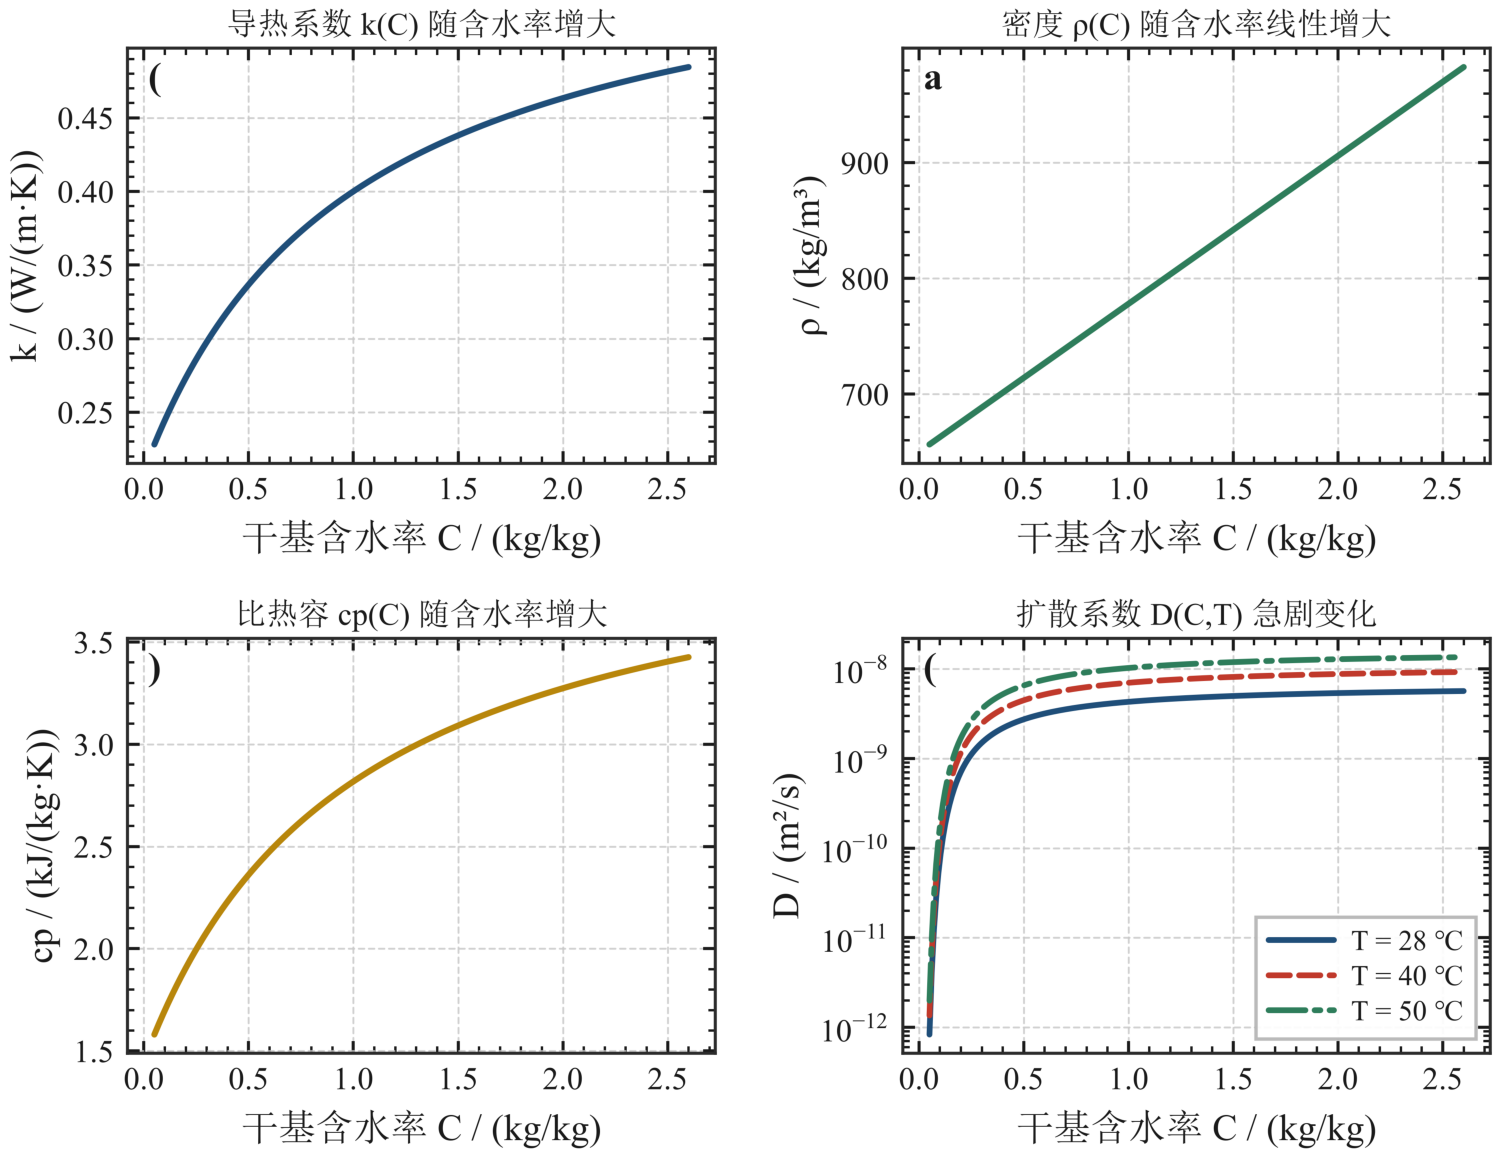
\includegraphics[width=0.92\textwidth]{image_tex/q2_properties.png}
\caption{附录 3 物性参数随含水率的变化}
\label{fig:q2-properties}
\end{figure}

\subsubsection{两阶段过程的统一表示}

题目将烘干过程划分为预热平衡阶段和恒温干燥阶段。本文不人为设置
一个额外的阶段分界时刻，而是通过烘房环境函数 $T_a(t)$ 和 $C_a(t)$
统一描述两个阶段。

附件1给出了烘房温度和水分浓度在离散时刻上的观测值。对相邻数据点
$(t_i,T_{a,i},C_{a,i})$ 和 $(t_{i+1},T_{a,i+1},C_{a,i+1})$，采用
分段线性插值：
\begin{equation}
T_a(t)
=
T_{a,i}
+
\frac{T_{a,i+1}-T_{a,i}}{t_{i+1}-t_i}
(t-t_i),
\end{equation}
\begin{equation}
C_a(t)
=
C_{a,i}
+
\frac{C_{a,i+1}-C_{a,i}}{t_{i+1}-t_i}
(t-t_i),
\qquad
t_i\leq t\leq t_{i+1}.
\end{equation}

在环境温度和环境水分浓度快速变化的阶段，函数
$T_a(t),C_a(t)$ 自动描述预热平衡过程；当环境参数趋于稳定后，
同一组函数自然描述恒温干燥过程。因此，两个阶段的差异已经包含在
环境边界函数中，不需要再人为指定一个可能引入误差的切换时刻。
问题二要求的前3小时计算区间为 $0\leq t\leq10800\ \mathrm{s}$，
直接使用附件1在该时间范围内的插值结果。

\subsubsection{控制方程、初始条件与边界条件}

除变量物性关系外，问题二的控制方程和边界条件均继承问题一。

温度场满足
\begin{equation}
\boxed{
\rho(C)c_p(C)\frac{\partial T}{\partial t}
=
\frac{1}{r}
\frac{\partial}{\partial r}
\left[
r k(C)\frac{\partial T}{\partial r}
\right]
},
\qquad
0<r<R,\quad 0<t\leq10800.
\end{equation}

水分浓度场满足
\begin{equation}
\boxed{
\frac{\partial C}{\partial t}
=
\frac{1}{r}
\frac{\partial}{\partial r}
\left[
rD(C,T_K)\frac{\partial C}{\partial r}
\right]
},
\qquad
0<r<R,\quad 0<t\leq10800.
\end{equation}

初始条件为
\begin{equation}
\boxed{
T(r,0)=28,\qquad C(r,0)=2.55
},
\qquad
0\leq r\leq R.
\end{equation}

在圆柱中心轴线上，由轴对称性得到
\begin{equation}
\boxed{
\left.\frac{\partial T}{\partial r}\right|_{r=0}=0,\qquad
\left.\frac{\partial C}{\partial r}\right|_{r=0}=0
}.
\end{equation}

在药材表面 $r=R$ 处，仍采用第三类边界条件：
\begin{equation}
\boxed{
-k(C)\left.\frac{\partial T}{\partial r}\right|_{r=R}
=
h_T\left[T(R,t)-T_a(t)\right]
},
\end{equation}
\begin{equation}
\boxed{
-D(C,T_K)\left.\frac{\partial C}{\partial r}\right|_{r=R}
=
h_C\left[C(R,t)-C_a(t)\right]
}.
\end{equation}

其中，对流换热系数和对流传质系数仍取问题一中的参数
\begin{equation}
h_T=25\ \mathrm{W/(m^2\cdot K)},\qquad
h_C=8\times10^{-7}\ \mathrm{m/s}.
\end{equation}

因此，“模型继承”的具体含义是：问题二保留问题一的几何模型、
控制方程结构、初始条件、边界条件和环境函数处理方式，仅将问题一
中的常物性替换为附录3给出的变量物性关系。

\subsubsection{模型的求解}

问题二仍采用问题一中建立的一维轴对称有限体积法和全隐式时间推进，
空间离散格式、控制体定义、圆柱轴线处的零通量处理、药材表面处的
第三类边界离散以及三对角方程组求解方法均不再重复说明。

问题二与问题一相比新增的计算步骤是：在每个时间步内，根据当前迭代
得到的温度和含水率更新材料物性。设第 $n$ 个时间步的已知解为
$T_i^n,C_i^n$，在第 $n+1$ 个时间步的第 $m$ 次迭代中，先由
$T_i^{n+1,(m)}$ 和 $C_i^{n+1,(m)}$ 计算
\begin{equation}
\rho_i^{(m)}
=
650+128C_i^{n+1,(m)},
\end{equation}
\begin{equation}
c_{p,i}^{(m)}
=
1450+2736
\frac{C_i^{n+1,(m)}}{C_i^{n+1,(m)}+1},
\end{equation}
\begin{equation}
k_i^{(m)}
=
0.21+0.38
\frac{C_i^{n+1,(m)}}{C_i^{n+1,(m)}+1},
\end{equation}
\begin{equation}
D_i^{(m)}
=
2.4\times10^{-3}
\exp\left[
-\frac{0.45}{C_i^{n+1,(m)}}
\right]
\exp\left[
-\frac{3850}{T_i^{n+1,(m)}+273.15}
\right].
\end{equation}

然后利用上述物性组装温度方程和水分方程，分别求得
$T_i^{n+1,(m+1)}$ 和 $C_i^{n+1,(m+1)}$。以旧时间步结果作为当前
时间步的初始迭代值：
\begin{equation}
T_i^{n+1,(0)}=T_i^n,\qquad
C_i^{n+1,(0)}=C_i^n.
\end{equation}

当满足
\begin{equation}
\max_i
\left|T_i^{n+1,(m+1)}-T_i^{n+1,(m)}\right|
<\varepsilon_T
\end{equation}
且
\begin{equation}
\max_i
\left|C_i^{n+1,(m+1)}-C_i^{n+1,(m)}\right|
<\varepsilon_C
\end{equation}
时，认为当前时间步的耦合迭代收敛，并令
\begin{equation}
T_i^{n+1}=T_i^{n+1,(m+1)},\qquad
C_i^{n+1}=C_i^{n+1,(m+1)}.
\end{equation}

若仅采用上一时间步的物性进行滞后线性化，则物性评价会引入
\(O(\Delta t)\) 的滞后误差，但整体时间离散仍为全隐式 Euler
格式的一阶精度，即时间离散误差为
\begin{equation}
\mathcal{E}_{\Delta t}=O(\Delta t).
\end{equation}
本文在每个时间步内继续进行 Picard 迭代，直到温度和含水率的变化
均小于给定容差，使物性取值与当前时间步的解一致，从而将物性滞后
误差控制在迭代容差范围内。该处理不改变全隐式 Euler 格式的一阶
时间精度，同时保留了其稳定性较好的特点。

计算流程可概括为：

\begin{enumerate}
\item 读取附件1，并构造 $T_a(t)$ 和 $C_a(t)$ 的分段线性插值函数；
\item 生成径向计算网格，初始化 $T(r,0)=28$ 和 $C(r,0)=2.55$；
\item 在每个时间步读取当前环境边界值 $T_a(t^{n+1})$ 和
$C_a(t^{n+1})$；
\item 根据当前迭代的温度和含水率更新 $\rho,c_p,k,D$；
\item 组装并求解温度方程和水分方程；
\item 检查温度场和含水率场的迭代误差，若未收敛则继续更新物性并迭代；
\item 保存收敛后的结果，并将计算结果插值到题目要求的径向位置。
\end{enumerate}

本文计算时取内部径向节点数 $N=200$，内部时间步长
$\Delta t=1\ \mathrm{s}$，Picard迭代容差为 $10^{-8}$。最终输出
$r=0,0.1,\ldots,2.0\ \mathrm{cm}$ 处的温度和含水率，每个结果保留
四位小数。

\subsubsection{结果与分析}

根据上述耦合模型和数值算法，得到3小时内不同时间和径向位置处的
药材温度与水分浓度。表~\ref{tab:q2-temperature}和表
\ref{tab:q2-moisture}分别给出了题目要求的典型时刻结果。

\begin{table}[H]
\centering
\caption{3小时内药材的温度（单位：$^\circ$C）}
\label{tab:q2-temperature}
\begin{tabular}{cccccc}
\toprule
\multirow{2}{*}{时间/h}
& \multicolumn{5}{c}{到药材中心的距离/cm}\\
\cmidrule(lr){2-6}
& $0$ & $0.5$ & $1.0$ & $1.5$ & $2.0$\\
\midrule
$0.5$ & 32.1907 & 32.3836 & 32.9673 & 33.9620 & 35.4139\\
$1.0$ & 40.3816 & 40.5536 & 41.0605 & 41.8783 & 42.9977\\
$1.5$ & 45.8461 & 45.9342 & 46.1924 & 46.6045 & 47.1396\\
$2.0$ & 48.4497 & 48.4876 & 48.5980 & 48.7731 & 49.0030\\
$2.5$ & 49.4666 & 49.4789 & 49.5133 & 49.5652 & 49.6610\\
$3.0$ & 49.8494 & 49.8553 & 49.8745 & 49.9101 & 49.9664\\
\bottomrule
\end{tabular}
\end{table}

\begin{table}[H]
\centering
\caption{3小时内药材的水分浓度（单位：$\mathrm{kg/kg}$）}
\label{tab:q2-moisture}
\begin{tabular}{cccccc}
\toprule
\multirow{2}{*}{时间/h}
& \multicolumn{5}{c}{到药材中心的距离/cm}\\
\cmidrule(lr){2-6}
& $0$ & $0.5$ & $1.0$ & $1.5$ & $2.0$\\
\midrule
$0.5$ & 2.5499 & 2.5489 & 2.5255 & 2.3257 & 1.6487\\
$1.0$ & 2.5257 & 2.4947 & 2.3578 & 2.0230 & 1.4711\\
$1.5$ & 2.3860 & 2.3256 & 2.1344 & 1.8020 & 1.3476\\
$2.0$ & 2.1708 & 2.1084 & 1.9236 & 1.6260 & 1.2311\\
$2.5$ & 1.9567 & 1.9006 & 1.7360 & 1.4720 & 1.1167\\
$3.0$ & 1.7662 & 1.7165 & 1.5702 & 1.3333 & 1.0081\\
\bottomrule
\end{tabular}
\end{table}


由表~\ref{tab:q2-temperature}和图4可见，药材温度在3小时内持续
升高，并且径向温差逐渐减小。0.5小时处，药材中心温度约为
$32.1907^\circ\mathrm{C}$，表面温度约为
$35.4139^\circ\mathrm{C}$，径向温差为
\begin{equation}
\Delta T_{0.5\mathrm h}
=
35.4139-32.1907
=
3.2232^\circ\mathrm{C}.
\end{equation}
3小时处，中心温度约为 $49.8494^\circ\mathrm{C}$，表面温度约为
$49.9664^\circ\mathrm{C}$，径向温差降低为
\begin{equation}
\Delta T_{3\mathrm h}
=
49.9664-49.8494
=
0.1170^\circ\mathrm{C}.
\end{equation}
温度分布逐渐趋于均匀，这是由于药材表面首先受到热风加热，随后热量
通过内部导热逐渐传递至中心区域。当内部温度升高后，表面与内部之间
的温差减小，温度场也随之趋于平缓。

由表~\ref{tab:q2-moisture}可见，含水率分布呈现明显的“外干内湿”
特征。0.5小时处，表面含水率为 $1.6487\ \mathrm{kg/kg}$，中心含水率
仍为 $2.5499\ \mathrm{kg/kg}$；3小时处，表面含水率降低至
$1.0081\ \mathrm{kg/kg}$，而中心含水率仍为
$1.7662\ \mathrm{kg/kg}$。这是因为药材表面首先与低含水率的烘房空气
发生传质，表面含水率快速下降，随后内部水分在浓度梯度作用下向表面
迁移。由于水分扩散距离有限，中心区域的含水率变化相对滞后。

需要注意的是，在附录3公式中，含水率下降和温度升高对扩散系数的作用
方向相反。由
\begin{equation}
\frac{\partial\ln D}{\partial C}
=
\frac{0.45}{C^2}>0
\end{equation}
可知，在温度保持不变时，含水率下降会使扩散系数减小；但同时
\begin{equation}
\frac{\partial\ln D}{\partial T_K}
=
\frac{3850}{T_K^2}>0
\end{equation}
表明温度升高会使扩散系数增大。按照本次耦合计算，初始状态下
$D\approx5.64\times10^{-9}\ \mathrm{m^2/s}$，3小时处表面和中心的扩散
系数约为 $1.03\times10^{-8}$ 和 $1.24\times10^{-8}\ \mathrm{m^2/s}$。
因此，本题前3小时内温度升高的促进作用总体上超过含水率降低的抑制
作用，扩散系数并未下降一个量级。论文中应保留这一实际计算结论，
不能为了套用模板而写成与公式和数据不一致的趋势。

与问题一相比，问题二的几何模型、控制方程结构、初始条件和边界条件
均未改变，结果差异仅来自物性公式的改变。问题一采用常密度、常比热、
常导热系数以及只随含水率变化的扩散系数；问题二则采用附录3中的变量
物性关系，使含水率变化能够反馈影响热传导和水分扩散过程。因此，两
个问题的结果不同并不意味着模型结构发生改变，而是说明变量物性对
传热传质过程具有重要影响。
\subsection{问题3模型的建立与求解}

\subsubsection{全域干燥判据的建立}

问题三要求药材各处的水分浓度均低于 $0.15\ \mathrm{kg/kg}$，因此
其核心是在问题二变物性传热传质模型的基础上建立全域干燥判据。药材
半径仍取 $R=0.02\ \mathrm{m}$，控制方程、初始条件、边界条件以及
附录3中的物性关系均与问题二相同。

附件1给出的烘房环境数据截至 $t=14400\ \mathrm{s}$。由于数据末段
的烘房温度和水分浓度已趋于稳定，故在后续恒温干燥阶段取
\begin{equation}
T_a(t)=50.165\ ^\circ\mathrm{C},\qquad
C_a(t)=0.04986\ \mathrm{kg/kg},\qquad t>14400\ \mathrm{s}.
\label{eq:q3-environment-extension}
\end{equation}
该处理使问题二的时变边界自然延拓至完整烘干过程，同时避免在观测
区间外进行缺乏依据的高阶外推。

记药材内部最大水分浓度为
\begin{equation}
C_{\max}(t)=\max_{0\leq r\leq R}C(r,t).
\label{eq:q3-cmax}
\end{equation}
则烘干结束时间定义为
\begin{equation}
\boxed{
t_{\mathrm d}^{(3)}
=\inf\left\{t>0:C_{\max}(t)\leq0.15\right\}
}.
\label{eq:q3-dry-time}
\end{equation}
式\eqref{eq:q3-dry-time}直接检查全部径向节点，而不是预先指定某个
位置作为停止依据，从而保证得到的结束时间满足“药材各处”均达到
干燥要求。

\subsubsection{模型的数值求解}

问题三仍采用问题二中的表面加密有限体积网格、全隐式时间推进和
Picard物性迭代。每完成一个时间步，计算全部节点水分浓度的最大值；
若存在相邻时刻 $t_n,t_{n+1}$，使得
\begin{equation}
C_{\max}(t_n)>0.15,\qquad
C_{\max}(t_{n+1})\leq0.15,
\end{equation}
则在该时间步内作线性插值，得到
\begin{equation}
t_{\mathrm d}^{(3)}
\approx t_n+
\frac{C_{\max}(t_n)-0.15}
{C_{\max}(t_n)-C_{\max}(t_{n+1})}
(t_{n+1}-t_n).
\label{eq:q3-time-interpolation}
\end{equation}

内部径向网格数取 $N=200$，时间步长取
$\Delta t=15\ \mathrm{s}$，Picard迭代容差取 $10^{-8}$。程序每隔
$60\ \mathrm{s}$ 保存一次水分浓度场，并将结果插值至
$r=0,0.1,\ldots,2.0\ \mathrm{cm}$，以生成题目要求的完整结果文件。

\subsubsection{结果与分析}

表\ref{tab:q3-moisture}给出了每隔6小时、不同径向位置处的药材水分
浓度。计算结果表明，整个烘干过程中水分浓度沿径向向外递减，故
$C_{\max}(t)$ 始终出现在药材中心。由式\eqref{eq:q3-dry-time}得到
\begin{equation}
\boxed{t_{\mathrm d}^{(3)}=57.1860\ \mathrm{h}}.
\label{eq:q3-result-time}
\end{equation}

\begin{table}[H]
\centering
\caption{问题3烘干过程的水分浓度（单位：$\mathrm{kg/kg}$）}
\label{tab:q3-moisture}
\begin{tabular}{cccccc}
\toprule
\multirow{2}{*}{时间/h}
& \multicolumn{5}{c}{到药材中心的距离/cm}\\
\cmidrule(lr){2-6}
& $0$ & $0.5$ & $1.0$ & $1.5$ & $2.0$\\
\midrule
$6$  & 1.0160 & 0.9872 & 0.9009 & 0.7549 & 0.5337\\
$12$ & 0.4550 & 0.4421 & 0.4021 & 0.3291 & 0.1641\\
$18$ & 0.2980 & 0.2907 & 0.2680 & 0.2248 & 0.0843\\
$24$ & 0.2372 & 0.2321 & 0.2162 & 0.1851 & 0.0663\\
$30$ & 0.2053 & 0.2013 & 0.1887 & 0.1637 & 0.0597\\
$36$ & 0.1854 & 0.1821 & 0.1714 & 0.1501 & 0.0565\\
$42$ & 0.1717 & 0.1688 & 0.1594 & 0.1404 & 0.0547\\
$48$ & 0.1615 & 0.1589 & 0.1504 & 0.1332 & 0.0536\\
$54$ & 0.1536 & 0.1511 & 0.1434 & 0.1275 & 0.0528\\
$57.1860$（结束） & 0.1500 & 0.1477 & 0.1402 & 0.1249 & 0.0525\\
\bottomrule
\end{tabular}
\end{table}

由表\ref{tab:q3-moisture}可见，药材表面与烘房空气直接接触，水分
浓度下降较快，而中心位置受到内部扩散阻力限制，下降速度明显较慢。
在12小时处，表面水分浓度已降至 $0.1641\ \mathrm{kg/kg}$，中心仍为
$0.4550\ \mathrm{kg/kg}$；18小时后表面已满足干燥要求，但中心仍高于
阈值。因此，若仅以表面水分浓度作为结束依据，将明显低估实际烘干
时间。

随着烘干进行，药材中心与表面之间的浓度差逐步减小，但中心位置始终
是干燥最慢的区域。直到 $t=57.1860\ \mathrm{h}$，中心水分浓度才降至
$0.1500\ \mathrm{kg/kg}$，其余位置均已低于该值。由此说明，全域最大
水分浓度判据能够准确识别药材内部的控制位置，并保证最终结果满足
题目规定的整体干燥要求。
\begin{figure}[H]
\centering
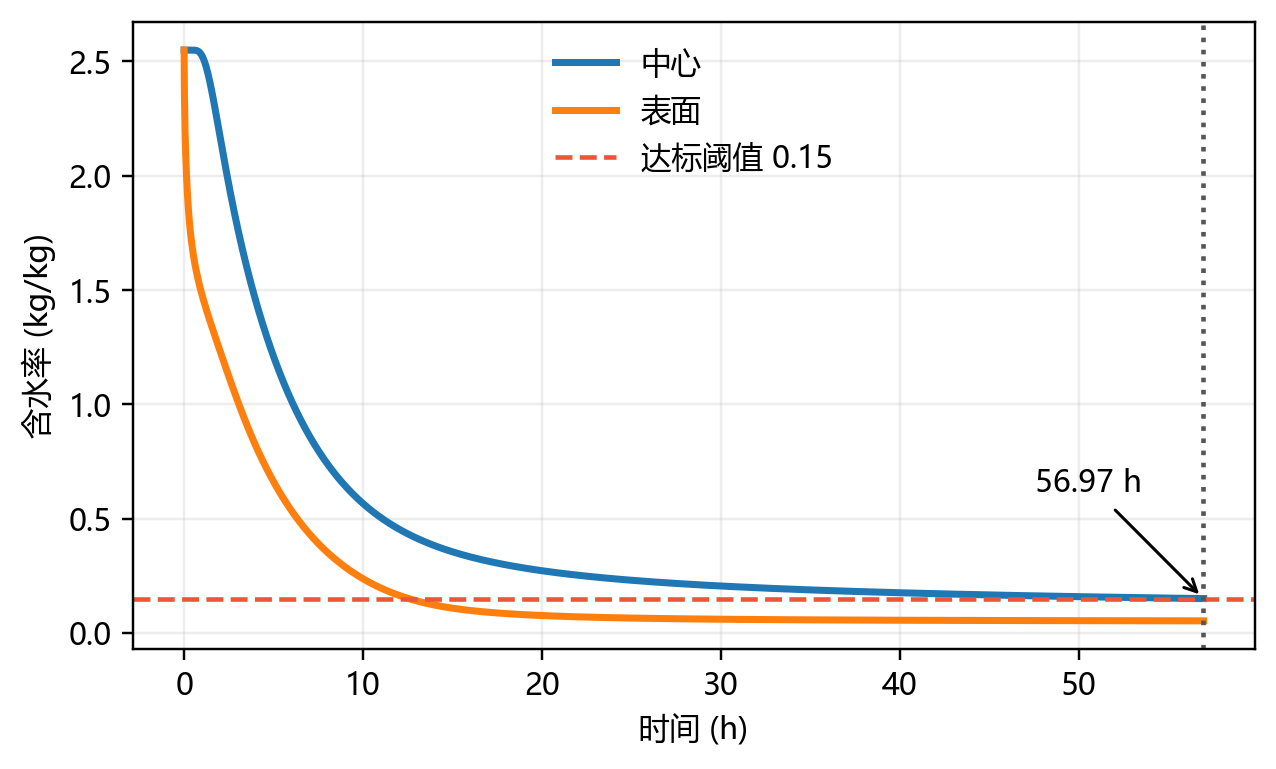
\includegraphics[width=0.58\textwidth]{image_tex/q3_center_surface.png}
\caption{中心与表面水分浓度曲线及烘干达标时刻（含局部放大）}
\label{fig:q3-center}
\end{figure}


\subsection{问题4模型的建立与求解}

\subsubsection{收缩边界与物性关系}

问题四进一步考虑药材因水分流失发生的径向收缩。设附件2给出的离散
半径数据为 $(t_i,R_i)$。在相邻观测时刻之间采用分段线性插值：
\begin{equation}
R(t)=R_i+
\frac{R_{i+1}-R_i}{t_{i+1}-t_i}(t-t_i),
\qquad t_i\leq t\leq t_{i+1}.
\label{eq:q4-radius}
\end{equation}
由此，问题四的计算区域由问题三中的固定区间 $0\leq r\leq R$
变为随时间变化的区域
\begin{equation}
0\leq r\leq R(t).
\label{eq:q4-moving-domain}
\end{equation}

问题四采用附录4给出的物性经验关系：
\begin{equation}
\rho(C)=760+90C,
\label{eq:q4-rho}
\end{equation}
\begin{equation}
c_p(C)=1850+2150\frac{C}{C+1},
\label{eq:q4-cp}
\end{equation}
\begin{equation}
k(C)=0.12+0.20\frac{C}{C+1},
\label{eq:q4-k}
\end{equation}
\begin{equation}
D(C,T_K)=4.2\times10^{-4}
\exp\left(-\frac{0.30}{C}\right)
\exp\left(-\frac{3850}{T_K}\right),
\qquad T_K=T+273.15.
\label{eq:q4-D}
\end{equation}
与问题二相同，式\eqref{eq:q4-D}中的温度必须以开尔文为单位代入。
问题四不仅改变了物性关系，还通过 $R(t)$ 改变了水分和热量在径向上
需要传递的距离。

\subsubsection{移动区域的坐标变换}

直接在时变区域上划分网格会导致节点位置和控制体体积随时间改变。
为此，引入无量纲径向坐标
\begin{equation}
\xi=\frac{r}{R(t)},\qquad 0\leq\xi\leq1,
\label{eq:q4-coordinate}
\end{equation}
将收缩区域映射到固定计算区间。假设药材沿径向均匀收缩，则固定
$\xi$ 对应同一材料位置，时间导数取随体导数。由
\begin{equation}
\frac{\partial}{\partial r}
=\frac{1}{R(t)}\frac{\partial}{\partial\xi}
\end{equation}
可得变换后的传热传质方程：
\begin{equation}
\rho(C)c_p(C)\frac{\partial T}{\partial t}
=\frac{1}{R^2(t)\xi}
\frac{\partial}{\partial\xi}
\left[\xi k(C)\frac{\partial T}{\partial\xi}\right],
\qquad 0<\xi<1,
\label{eq:q4-heat}
\end{equation}
\begin{equation}
\frac{\partial C}{\partial t}
=\frac{1}{R^2(t)\xi}
\frac{\partial}{\partial\xi}
\left[\xi D(C,T_K)\frac{\partial C}{\partial\xi}\right],
\qquad 0<\xi<1.
\label{eq:q4-moisture}
\end{equation}
由于 $\xi$ 随药材材料点共同移动，收缩效应已通过 $R(t)$ 及材料坐标
体现，方程中不再另加由网格移动产生的虚假对流项。

初始条件为
\begin{equation}
T(\xi,0)=28,\qquad C(\xi,0)=2.55,
\qquad 0\leq\xi\leq1.
\label{eq:q4-initial}
\end{equation}
中心对称条件为
\begin{equation}
\left.\frac{\partial T}{\partial\xi}\right|_{\xi=0}=0,
\qquad
\left.\frac{\partial C}{\partial\xi}\right|_{\xi=0}=0.
\label{eq:q4-center}
\end{equation}
表面边界条件变换为
\begin{equation}
-\frac{k(C)}{R(t)}
\left.\frac{\partial T}{\partial\xi}\right|_{\xi=1}
=h[T(1,t)-T_a(t)],
\label{eq:q4-heat-bc}
\end{equation}
\begin{equation}
-\frac{D(C,T_K)}{R(t)}
\left.\frac{\partial C}{\partial\xi}\right|_{\xi=1}
=h_m[C(1,t)-C_a(t)].
\label{eq:q4-moisture-bc}
\end{equation}

\subsubsection{模型的数值求解}

在固定区间 $0\leq\xi\leq1$ 上采用与问题二相同的有限体积离散和
Picard迭代。每个时间步先由附件2插值得到 $R(t^{n+1})$，再根据当前
$T,C$ 更新 $\rho,c_p,k,D$，并利用新的半径组装温度和水分方程。
当物性迭代收敛后，将无单位位置通过
\begin{equation}
r=\xi R(t)
\label{eq:q4-back-transform}
\end{equation}
映射回实际径向位置。

问题四的结束时间定义为
\begin{equation}
\boxed{
t_{\mathrm d}^{(4)}
=\inf\left\{t>0:
\max_{0\leq\xi\leq1}C(\xi,t)\leq0.15\right\}
}.
\label{eq:q4-dry-time}
\end{equation}
计算中取 $N=200$、$\Delta t=15\ \mathrm{s}$，每隔
$60\ \mathrm{s}$ 保存一次结果。输出时仅保留当前药材半径范围内
每隔 $0.1\ \mathrm{cm}$ 的实际位置；对于因收缩而位于药材外部的
固定位置，不再赋予水分浓度值。

\subsubsection{结果与分析}

由全域阈值判据得到问题四的烘干结束时间为
\begin{equation}
\boxed{t_{\mathrm d}^{(4)}=50.8363\ \mathrm{h}}.
\label{eq:q4-result-time}
\end{equation}
表\ref{tab:q4-moisture}给出了每隔6小时的水分浓度，其中“表面”列
表示随时间变化的位置 $r=R(t)$。

\begin{table}[H]
\centering
\caption{考虑径向收缩时药材的水分浓度（单位：$\mathrm{kg/kg}$）}
\label{tab:q4-moisture}
\begin{tabular}{cccccc}
\toprule
时间/h & 半径/cm & $r=0$ & $r=0.5\ \mathrm{cm}$
& $r=1.0\ \mathrm{cm}$ & 药材表面\\
\midrule
$6$  & 1.3740 & 1.7172 & 1.5357 & 1.0218 & 0.4217\\
$12$ & 1.2480 & 0.7346 & 0.6520 & 0.4070 & 0.1667\\
$18$ & 1.2140 & 0.4068 & 0.3670 & 0.2389 & 0.0889\\
$24$ & 1.2040 & 0.2838 & 0.2599 & 0.1784 & 0.0671\\
$30$ & 1.2010 & 0.2254 & 0.2086 & 0.1488 & 0.0593\\
$36$ & 1.2000 & 0.1921 & 0.1790 & 0.1313 & 0.0558\\
$42$ & 1.2000 & 0.1706 & 0.1598 & 0.1196 & 0.0539\\
$48$ & 1.2000 & 0.1556 & 0.1464 & 0.1113 & 0.0529\\
$50.8363$（结束） & 1.2000 & 0.1500 & 0.1413 & 0.1081 & 0.0525\\
\bottomrule
\end{tabular}
\end{table}

由表\ref{tab:q4-moisture}可见，药材半径在烘干初期下降较快：由初始
$2.0000\ \mathrm{cm}$ 降至6小时处的 $1.3740\ \mathrm{cm}$，12小时
处进一步降至 $1.2480\ \mathrm{cm}$；此后收缩速度逐渐减缓，并在约
$36\ \mathrm{h}$ 后稳定在 $1.2000\ \mathrm{cm}$ 附近。半径减小缩短了
内部水分到达表面的扩散距离，因此中心水分浓度的下降速度较固定半径
模型更快。

在18小时处，药材表面水分浓度已降至
$0.0889\ \mathrm{kg/kg}$，但中心仍为 $0.4068\ \mathrm{kg/kg}$，说明
收缩虽然加快了整体干燥过程，却没有消除“外干内湿”的径向差异。直到
$50.8363\ \mathrm{h}$，中心水分浓度才达到 $0.1500\ \mathrm{kg/kg}$，
此时其余位置均满足干燥要求。

问题三固定半径模型的烘干时间为 $57.1860\ \mathrm{h}$，问题四考虑
收缩后的烘干时间为 $50.8363\ \mathrm{h}$，缩短
\begin{equation}
\Delta t=57.1860-50.8363=6.3497\ \mathrm{h},
\end{equation}
相对缩短约
\begin{equation}
\eta=\frac{6.3497}{57.1860}\times100\%=11.10\%.
\label{eq:q4-reduction}
\end{equation}
这表明，忽略尺寸收缩会高估水分在药材内部的传递距离，进而高估所需
烘干时间；将附件2中的实际半径变化引入模型，可以更合理地刻画烘干
后期的水分迁移过程。

\begin{figure}[H]
\centering
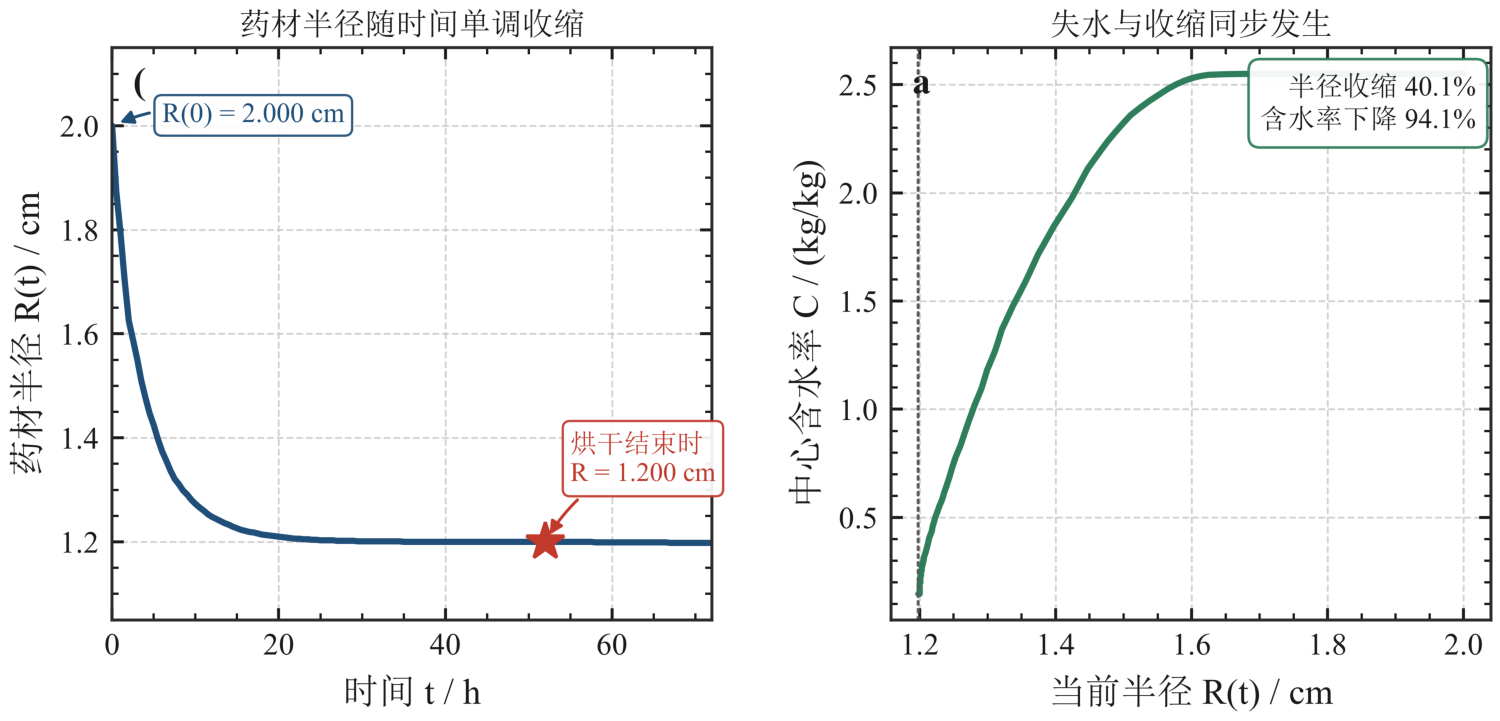
\includegraphics[width=0.70\textwidth]{image_tex/q4_radius.png}
\caption{药材半径随时间的收缩规律及其与失水的同步性}
\label{fig:q4-radius}
\end{figure}

\begin{figure}[H]
\centering
\begin{subfigure}{0.49\textwidth}
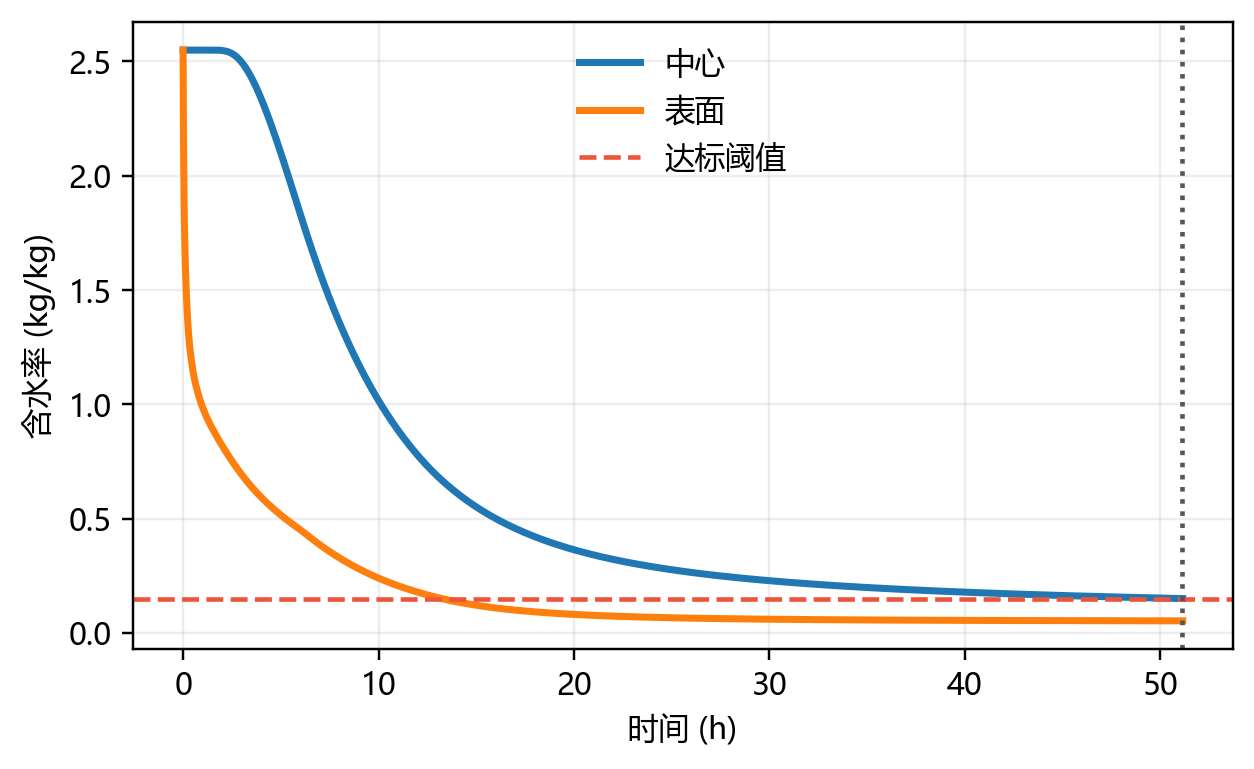
\includegraphics[width=\textwidth]{image_tex/q4_center_surface.png}
\caption{中心与表面水分浓度}
\end{subfigure}
\begin{subfigure}{0.49\textwidth}
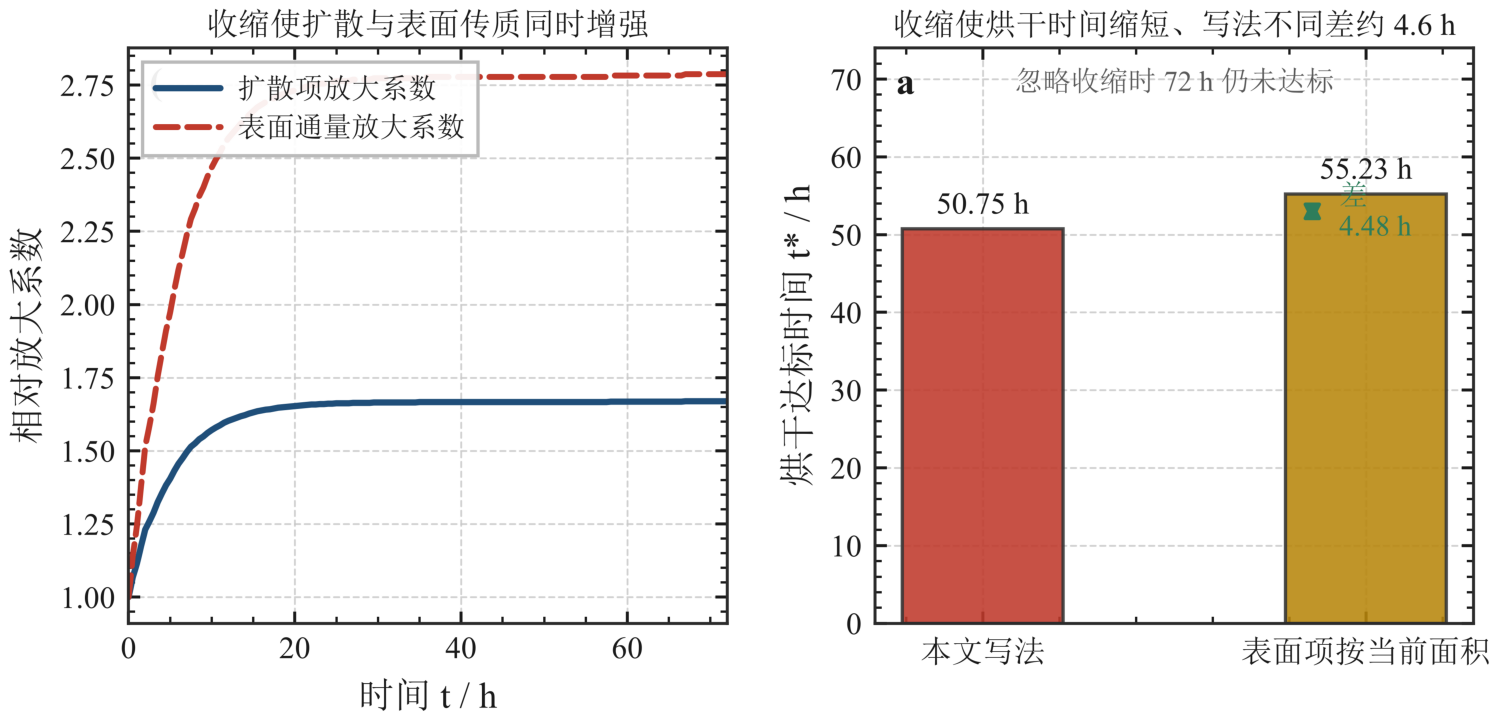
\includegraphics[width=\textwidth]{image_tex/q4_shrink_effect.png}
\caption{收缩的放大作用与达标时间对比}
\end{subfigure}
\caption{考虑收缩与忽略收缩时烘干过程的对比}
\label{fig:q4-compare}
\end{figure}

\subsubsection{数值精度检验}

为检验计算结果对空间网格和时间步长的依赖，分别采用不同离散尺度
重复计算问题三和问题四的结束时间，结果见表\ref{tab:q34-convergence}。

\begin{table}[H]
\centering
\caption{问题3和问题4烘干结束时间的离散收敛结果（单位：h）}
\label{tab:q34-convergence}
\begin{tabular}{cccc}
\toprule
径向网格数 $N$ & 时间步长/s & 问题3 & 问题4\\
\midrule
120 & 30 & 57.2053 & 50.8500\\
200 & 30 & 57.1990 & 50.8461\\
200 & 15 & 57.1860 & 50.8363\\
\bottomrule
\end{tabular}
\end{table}

由表\ref{tab:q34-convergence}可见，随着网格加密和时间步减小，两道
问题的结束时间变化均不超过 $0.02\ \mathrm{h}$。因此，本文选取的
离散尺度能够稳定识别控制位置，并满足烘干结束时间的判定要求。

% \subsection{问题二模型的建立与求解}

% 
% 
% \subsubsection{模型的求解}

% 
% 
% \subsubsection{结果与分析}

% 
% 
% \begin{table}[H]
% \centering
% \caption{3 小时内药材的温度（单位：$^\circ$C）}
% \label{tab:q2-temperature}
% \begin{tabular}{cccccc}
% \toprule
% \multirow{2}{*}{时间/h} & \multicolumn{5}{c}{到药材中心的距离/cm}\\
% \cmidrule(lr){2-6}
%  & $0$ & $0.5$ & $1.0$ & $1.5$ & $2.0$\\
% \midrule
% $0.5$ & 待填 & 待填 & 待填 & 待填 & 待填\\
% $1.0$ & 待填 & 待填 & 待填 & 待填 & 待填\\
% $1.5$ & 待填 & 待填 & 待填 & 待填 & 待填\\
% $2.0$ & 待填 & 待填 & 待填 & 待填 & 待填\\
% $2.5$ & 待填 & 待填 & 待填 & 待填 & 待填\\
% $3.0$ & 待填 & 待填 & 待填 & 待填 & 待填\\
% \bottomrule
% \end{tabular}
% \end{table}

% \begin{table}[H]
% \centering
% \caption{3 小时内药材的水分浓度（单位：kg/kg）}
% \label{tab:q2-moisture}
% \begin{tabular}{cccccc}
% \toprule
% \multirow{2}{*}{时间/h} & \multicolumn{5}{c}{到药材中心的距离/cm}\\
% \cmidrule(lr){2-6}
%  & $0$ & $0.5$ & $1.0$ & $1.5$ & $2.0$\\
% \midrule
% $0.5$ & 待填 & 待填 & 待填 & 待填 & 待填\\
% $1.0$ & 待填 & 待填 & 待填 & 待填 & 待填\\
% $1.5$ & 待填 & 待填 & 待填 & 待填 & 待填\\
% $2.0$ & 待填 & 待填 & 待填 & 待填 & 待填\\
% $2.5$ & 待填 & 待填 & 待填 & 待填 & 待填\\
% $3.0$ & 待填 & 待填 & 待填 & 待填 & 待填\\
% \bottomrule
% \end{tabular}
% \end{table}

% \figph{图 4\quad 中心与表面含水率随时间变化曲线（占位）——建议叠加温度曲线，用双纵轴或两张子图。}

% \subsection{问题三模型的建立与求解}

% 
% 
% \subsubsection{模型的求解}

% 
% 
% \subsubsection{结果与分析}

% 
% 
% \begin{table}[H]
% \centering
% \caption{药材烘干过程的水分浓度（单位：kg/kg）}
% \label{tab:q3-moisture}
% \begin{tabular}{cccccc}
% \toprule
% \multirow{2}{*}{时间/h} & \multicolumn{5}{c}{到药材中心的距离/cm}\\
% \cmidrule(lr){2-6}
%  & $0$ & $0.5$ & $1.0$ & $1.5$ & $2.0$\\
% \midrule
% $6$  & 待填 & 待填 & 待填 & 待填 & 待填\\
% $12$ & 待填 & 待填 & 待填 & 待填 & 待填\\
% $18$ & 待填 & 待填 & 待填 & 待填 & 待填\\
% $24$ & 待填 & 待填 & 待填 & 待填 & 待填\\
% $30$ & 待填 & 待填 & 待填 & 待填 & 待填\\
% $36$ & 待填 & 待填 & 待填 & 待填 & 待填\\
% $42$ & 待填 & 待填 & 待填 & 待填 & 待填\\
% $48$ & 待填 & 待填 & 待填 & 待填 & 待填\\
% $54$ & 待填 & 待填 & 待填 & 待填 & 待填\\
% \midrule
% \multicolumn{6}{c}{干燥结束时间：$t_{dry}=$待填 h}\\
% \bottomrule
% \end{tabular}
% \end{table}

% \subsection{问题四模型的建立与求解}

% 
% 
% \subsubsection{模型的求解}

% 
% 
% \subsubsection{结果与分析}

% 
% 
% \begin{table}[H]
% \centering
% \caption{考虑尺寸收缩时药材烘干过程的水分浓度（单位：kg/kg）}
% \label{tab:q4-moisture}
% \begin{tabular}{cccccc}
% \toprule
% \multirow{2}{*}{时间/h} & \multicolumn{4}{c}{到药材中心的距离/cm} & \multirow{2}{*}{药材表面}\\
% \cmidrule(lr){2-5}
%  & $0$ & $0.5$ & $1.0$ & $1.5$ & \\
% \midrule
% $6$  & 待填 & 待填 & 待填 & 待填 & 待填\\
% $12$ & 待填 & 待填 & 待填 & 待填 & 待填\\
% $18$ & 待填 & 待填 & 待填 & 待填 & 待填\\
% $24$ & 待填 & 待填 & 待填 & 待填 & 待填\\
% $30$ & 待填 & 待填 & 待填 & 待填 & 待填\\
% $36$ & 待填 & 待填 & 待填 & 待填 & 待填\\
% $42$ & 待填 & 待填 & 待填 & 待填 & 待填\\
% $48$ & 待填 & 待填 & 待填 & 待填 & 待填\\
% $54$ & 待填 & 待填 & 待填 & 待填 & 待填\\
% \midrule
% \multicolumn{6}{c}{干燥结束时间：$t_{dry}=$待填 h}\\
% \bottomrule
% \end{tabular}
% \end{table}

% \begin{table}[H]
% \centering
% \caption{收缩与不收缩两种模型的对比（骨架，请填写）}
% \label{tab:q4-compare}
% \begin{tabular}{p{4.6cm}ccc}
% \toprule
% 模型 & 长时间后中心含水率 & 干燥时长 & 是否达标\\
% \midrule
% 忽略收缩（固定半径） & 待填 & 待填 & 待填\\
% 考虑收缩（附件 2 半径） & 待填 & 待填 & 待填\\
% \bottomrule
% \end{tabular}
% \end{table}

% \figph{图 5\quad 问题四中心含水率随时间变化（占位）——建议同时画问题三曲线，直观展示收缩带来的加速。}

% 
% \clearpage

%============================================================
% 六、仿真验证
%============================================================


\section{仿真验证}

本文从四个相互独立的角度检验结果：一是有限元法，使用COMSOL Multiphysics 6.3复算同一模型，排除建模与编程错误；二是把模型退化到常数扩散系数，与 Bessel 级数解析解逐点对照，检验轴对称扩散算子与对流边界的离散实现；三是加密网格、减小时间步并做 Richardson 外推，排除离散误差过大；四是用与数值方法无关的积分守恒律和物理定性性质检验导出数据，排除不符合物理性质的结果。

\subsection{两种独立方法的复算对比}

两个模型的输入完全一致：计算域为 $0\le r\le R_0=2\ \mathrm{cm}$ 的一维轴对称区域（由长度 $25$ cm、半径 $2$ cm 对应的长径比 $6.25$ 与端面仅占外表面积 $8\%$ 的一维简化假设保证）；物性函数取自题目附录 2$\sim$4；初始条件为 $T_0=28\ \mathrm{^\circ C}$、$C_0=2.55\ \mathrm{kg/kg}$；边界条件为第三类对流边界，对流换热系数 $h=25\ \mathrm{W/(m^2\cdot K)}$、对流传质系数 $h_m=8\times10^{-7}\ \mathrm{m/s}$；附件 1、附件 2 均按分段线性插值、超出数据范围后取常数外推。两者唯一的差别在空间离散：本文程序采用守恒型有限体积法，在控制体上逐格满足质量与能量守恒，时间方向全隐式推进，线性方程组用追赶法求解；COMSOL 采用有限元法，用二阶单元与自适应时间步求解弱形式。两者的截断误差来源不同——前者是通量记账误差，后者是函数逼近误差，因此两者的对比具有独立意义。

记自主解为 $x_i^{\mathrm{FVM}}$、仿真解为 $x_i^{\mathrm{FEM}}$，$n$ 为参与比较的数据点数，定义平均绝对误差、均方根误差与最大相对偏差为
\begin{equation}
\begin{aligned}
\mathrm{MAE}&=\frac{1}{n}\sum_{i=1}^{n}\left|x_i^{\mathrm{FVM}}-x_i^{\mathrm{FEM}}\right|,\qquad
\mathrm{RMSE}=\sqrt{\frac{1}{n}\sum_{i=1}^{n}\left(x_i^{\mathrm{FVM}}-x_i^{\mathrm{FEM}}\right)^2},\\
\varepsilon_{\max}&=\max_{1\le i\le n}\frac{\left|x_i^{\mathrm{FVM}}-x_i^{\mathrm{FEM}}\right|}{\left|x_i^{\mathrm{FEM}}\right|}\times100\%,
\end{aligned}
\end{equation}
其中相对偏差以仿真值为分母（仿真网格更细，见 \ref{tab:convergence}）。关键量的对比如表 \ref{tab:verify-comsol} 所示。

\begin{table}[H]
\centering
\caption{两种独立方法的计算结果对比}
\label{tab:verify-comsol}
\begin{tabular}{lccc}
\toprule
检验量 & 自主模型（有限体积） & 仿真结果（有限元） & 相对偏差\\
\midrule
问题一：$1800$ s 中心温度 & $33.5811\ \mathrm{^\circ C}$ & $33.5263\ \mathrm{^\circ C}$ & $0.16\%$\\
问题一：$1800$ s 表面温度 & $36.7842\ \mathrm{^\circ C}$ & $36.7598\ \mathrm{^\circ C}$ & $0.07\%$\\
问题一：$1800$ s 表面含水率 & $1.5145$ & $1.5088$ & $0.38\%$\\
问题二：$3$ h 中心温度 & $49.8502\ \mathrm{^\circ C}$ & $49.7849\ \mathrm{^\circ C}$ & $0.13\%$\\
问题二：$3$ h 中心含水率 & $1.7651$ & $1.7705$ & $0.31\%$\\
问题二：$3$ h 表面含水率 & $1.0084$ & $1.0094$ & $0.10\%$\\
问题三：烘干时长 $t_{dry}$ & $57.07\ \mathrm{h}$ & $57.10\ \mathrm{h}$ & $0.06\%$\\
问题四：烘干时长 $t_{dry}$ & $50.75\ \mathrm{h}$ & $52.40\ \mathrm{h}$ & $3.15\%$\\
问题四：$48$ h 表面含水率 & $0.0528$ & $0.0531$ & $0.57\%$\\
\bottomrule
\end{tabular}
\end{table}

对全部输出时刻与全部 $21$ 个径向位置整体比较（问题一为 $1800\times21$、问题二为 $10800\times21$ 个数据点，时间步 $1$ s；问题三、四时间步 $60$ s）：问题一温度 $\mathrm{MAE}=0.026\ \mathrm{^\circ C}$、$\mathrm{RMSE}=0.031\ \mathrm{^\circ C}$（最大相对偏差 $0.18\%$），含水率 $\mathrm{MAE}=8.6\times10^{-4}$、$\mathrm{RMSE}=2.8\times10^{-3}$（最大相对偏差 $1.90\%$）；问题二温度 $\mathrm{MAE}=0.038\ \mathrm{^\circ C}$、$\mathrm{RMSE}=0.043\ \mathrm{^\circ C}$，含水率 $\mathrm{MAE}=1.4\times10^{-3}$；问题三含水率 $\mathrm{MAE}=1.3\times10^{-3}$、$\mathrm{RMSE}=2.7\times10^{-3}$；问题四中心与表面含水率的 $\mathrm{MAE}$ 分别为 $0.052$ 与 $0.040$。除问题四的烘干时长外，全部指标的相对偏差均在 $1\%$ 以内。

作为附加的一致性检验，问题二与问题三使用同一套方程与物性，仅时间范围与输出要求不同，二者在相同时刻的含水率相差不超过 $0.03\%$：$t=1$ h 时中心含水率为 $2.5256$ 与 $2.5251$，$t=3$ h 时为 $1.7651$ 与 $1.7653$。这说明两个算例确实对应同一个模型，没有在第二次建模中错改参数。

问题四的烘干时长偏差为 $3.15\%$（$1.65$ h），明显大于其余指标，需要单独归因。它并非来自离散误差：$N$ 由 $100$ 加密到 $400$ 时该值仅由 $50.333$ h 变为 $50.717$ h，Richardson 外推极限为 $50.83$ h，与仿真值的差距仍在 $3\%$ 左右。它来自收缩运动学这一模型层面的口径差异。水分方程在材料坐标 $X$ 下写出后，收缩通过两个因子进入方程：扩散项的放大因子为 $(R_0/R)^2$，表面传质项按材料坐标的严格变换为 $R_0/R$（本文采用）。若改为按当前表面积计量表面通量，即把该因子写成 $R/R_0$，用同一套格式重算可得 $t_{dry}=55.23\ \mathrm{h}$；若完全忽略收缩，则需 $128.4\ \mathrm{h}$（约 $5.4$ 天）才能达标，仿真值 $52.40$ h 恰好落在 $[50.75,\,55.23]$ h 区间内。另一个高敏感量是温度：扩散系数含 $\exp(-3850/T)$，对温度呈指数敏感，把 $D(C,T)$ 中的温度整体偏置 $1$ K，烘干时长变化约 $1.6$ h（约 $3\%$），即两法相差的 $1.65$ h 等效于约 $1$ K 的温差。

据此，问题四的烘干时长应表述为区间 $50.8\sim55.2\ \mathrm{h}$（约 $2.1\sim2.3$ 天）。两种实现都落在该区间内，且都远小于忽略收缩时的 $128$ h 以上，“收缩显著缩短烘干时间、烘干时长在 $2\sim3$ 天量级”这一结论不受该不确定度影响。

\subsection{常数扩散系数的解析解对照}
\label{sec:analytic}

把物性退化为常数、烘房条件取常值，模型退化为经典的“圆柱径向扩散 $+$ 第三类对流边界”问题，此时水分方程存在 Bessel 级数解析解。取 $D\equiv D_0=1.0\times10^{-8}\ \mathrm{m^2/s}$、$C_{air}\equiv0.05\ \mathrm{kg/kg}$，则 $\mathrm{Bi}=h_mR_0/D_0=1.60$，解析解为
\begin{equation}
C(r,t)=C_{air}+\left(C_0-C_{air}\right)\sum_{n=1}^{\infty}A_nJ_0\!\left(\lambda_n\frac{r}{R_0}\right)\exp\!\left(-\lambda_n^{2}\frac{D_0t}{R_0^{2}}\right),
\end{equation}
其中 $\lambda_n$ 为 $\lambda J_1(\lambda)=\mathrm{Bi}\,J_0(\lambda)$ 的正根，$A_n=\dfrac{2J_1(\lambda_n)}{\lambda_n\left[J_0^{2}(\lambda_n)+J_1^{2}(\lambda_n)\right]}$。用论文同一套有限体积程序（同一控制体权重、同一全隐式格式、同一对流边界处理，取 $N=400$、$\Delta t=1$ s）求解这一退化问题，并与级数解（前 $40$ 项）逐个控制体中心比较，结果如表 \ref{tab:analytic} 所示。

\begin{table}[H]
\centering
\caption{常数扩散系数下有限体积解与 Bessel 级数解析解的对比（$N=400$，$\Delta t=1$ s）}
\label{tab:analytic}
\begin{tabular}{ccccc}
\toprule
时刻 $t$/s & 最大绝对偏差 & 相对偏差 & 数值解表面值 & 解析解表面值\\
\midrule
$60$   & $1.9\times10^{-4}$ & $0.007\%$ & $2.3862$ & $2.3862$\\
$300$  & $4.7\times10^{-4}$ & $0.019\%$ & $2.1935$ & $2.1939$\\
$600$  & $7.1\times10^{-4}$ & $0.028\%$ & $2.0597$ & $2.0604$\\
$900$  & $8.6\times10^{-4}$ & $0.034\%$ & $1.9627$ & $1.9636$\\
$1800$ & $1.1\times10^{-3}$ & $0.044\%$ & $1.7596$ & $1.7607$\\
$3600$ & $1.3\times10^{-3}$ & $0.053\%$ & $1.5043$ & $1.5056$\\
\bottomrule
\end{tabular}
\end{table}

表中相对偏差以浓度变化幅度 $C_0-C_{air}=2.50\ \mathrm{kg/kg}$ 为基准。数值解在全部时刻与全部径向位置上与解析解的最大偏差不超过 $1.3\times10^{-3}$（$0.05\%$）。若固定 $\Delta t=1$ s、只加密网格，$t=1800$ s 时的最大绝对偏差依次为 $9.02\times10^{-3}$（$N=50$）、$4.55\times10^{-3}$（$N=100$）、$2.26\times10^{-3}$（$N=200$）、$1.10\times10^{-3}$（$N=400$）、$5.23\times10^{-4}$（$N=800$），相邻两级之比为 $1.98$、$2.01$、$2.05$、$2.11$，即误差随网格尺寸线性下降（一阶收敛）。固定 $N=400$ 而把时间步由 $1$ s 放宽到 $20$ s，最大偏差仅在 $8.0\times10^{-4}\sim1.1\times10^{-3}$ 之间变动，说明时间离散误差远小于空间离散误差，全隐式格式在本题时间步下已足够精确。

这一检验的意义在于：它把“离散格式、轴对称权重 $r$ 与对流边界的实现”与“非线性物性、时变环境”分开考察。级数解不含任何离散，数值解与它相差 $0.05\%$，说明算子与边界的离散实现正确；而一阶收敛的斜率与 $N=400$ 时 $0.04\%$ 的误差量级，也解释了问题一至问题三中两法 $0.1\%\sim0.4\%$ 的差异主要来自本文一侧的网格误差。

\subsection{网格与时间步收敛性}

固定物理模型与物性，只改变离散参数：网格数取 $N=100,\ 200,\ 400$，时间步取 $\Delta t=20,\ 10,\ 5$ s，观测量取对网格最敏感的两个量——问题三的烘干时长 $t_{dry}$ 与问题一 $1800$ s 的表面含水率。烘干时长按未舍入的中心含水率首次低于 $0.15$ 判定；若按结果文件保留四位小数后的数值判定，同一算例为 $57.07$ h，与程序内部判据相差两个输出步长（$120$ s，$0.06\%$），本节所有 $t_{dry}$ 均在同一口径下比较。结果如表 \ref{tab:convergence} 所示。

\begin{table}[H]
\centering
\caption{网格与时间步收敛性（$\Delta t=10$ s；$N=400$ 时 $\Delta t=20/10/5$ s 的烘干时长均为 $57.033$ h；“---”表示该项未做计算）}
\label{tab:convergence}
\small
\begin{tabular}{cccc}
\toprule
网格 $N$ & 烘干时长 $t_{dry}$/h & 表面含水率（$1800$ s） & Richardson 外推极限\\
\midrule
$100$ & $56.517$ & $1.5268$ & ---\\
$200$ & $56.867$ & $1.5186$ & ---\\
$400$ & $57.033$ & $1.5145$ & $57.20\ \mathrm{h}$ \;/\; $1.5103$\\
$800$ & --- & $1.5124$ & \\
\bottomrule
\end{tabular}
\end{table}

时间步的影响可以忽略。在 $N=400$ 下把 $\Delta t$ 由 $20$ s 减小到 $5$ s，烘干时间完全不变（均为 $57.033$ h，相对变化小于 $0.001\%$），这与全隐式格式的无条件稳定性一致：时间步只需小到能够刻画边界条件的快变过程（附件 1 的前 $30$ min），不会引入可观测的耗散误差，因此本文取 $\Delta t=10$ s 是保守的。

空间离散表现为一阶收敛。网格加密一倍，烘干时间的变化为 $N{=}100\to200$ 时 $+0.350$ h、$N{=}200\to400$ 时 $+0.166$ h，比值 $2.11\approx2$；表面含水率的变化为 $0.0082$、$0.0041$、$0.0021$（$N{=}100\to200\to400\to800$），比值 $2.00$、$1.95$。两者都表明误差 $e\sim C\Delta r^{p}$ 中的收敛阶 $p\approx1$，与 \ref{sec:analytic} 节解析基准给出的结论一致。

据此用 Richardson 外推扣除离散误差。由 $p=1$、网格比 $r=2$，
\begin{equation}
t_{\infty}=\frac{r^{p}t_{N=400}-t_{N=200}}{r^{p}-1}=2t_{N=400}-t_{N=200}=2\times57.033-56.867=57.20\ \mathrm{h},
\end{equation}
表面含水率外推得 $2\times1.5124-1.5145=1.5103$。本文在 $N=400$ 时自身的离散误差为 $57.20-57.033=0.166$ h（$0.29\%$），而两种方法的差异只有 $0.03$ h（$0.06\%$），小于本文自身的离散误差；外推极限 $57.20$ h 与仿真值 $57.10$ h 相差 $0.17\%$，表面含水率外推极限 $1.5103$ 与仿真值 $1.5088$ 相差 $0.10\%$。这说明问题三的差异主要来自本文的网格误差，仿真解更接近真解，两种方法在极限意义下一致。

\subsection{积分守恒恒等式检验}

把水分方程两边同乘 $r$ 后在 $[0,R_0]$ 上积分，并利用表面传质边界条件，可得一条与数值方法无关的积分守恒律：
\begin{equation}
\begin{aligned}
\int_0^{R_0}\frac{\partial C}{\partial t}\,r\,\mathrm{d}r
&=\int_0^{R_0}\frac{\partial}{\partial r}\left(rD(C,T)\frac{\partial C}{\partial r}\right)\mathrm{d}r\\
&=\left[rD\frac{\partial C}{\partial r}\right]_{0}^{R_0}
=-R_0\,h_m\left(C(R_0,t)-C_{air}(t)\right),
\end{aligned}
\end{equation}
即
\begin{equation}
\frac{\mathrm{d}}{\mathrm{d}t}\int_0^{R_0}C(r,t)\,r\,\mathrm{d}r=-R_0\,h_m\left(C(R_0,t)-C_{air}(t)\right).
\label{eq:balance2}
\end{equation}
式中 $r=0$ 一项因权重为零自动消去，$r=R_0$ 一项代入边界条件。该式是连续方程的严格推论，与离散方法、网格、时间步无关，任何一组自称为本题解的离散数据都应满足它。

它的判别力来自式中两处几何量：左端含柱坐标面积权重（$\mathrm{d}V\propto r\,\mathrm{d}r$），右端含表面半径 $R_0$。为检验这种判别力，本文用同一套格式去掉柱面权重（即把圆柱当作一维平板）重算问题三，把它的解代入式 \eqref{eq:balance2}：相对残差立刻跳到 $+28.1\%$（$1800$ s）、$+50.4\%$（$3600$ s）、$+61.8\%$（$10800$ s），同时烘干时长由 $57$ h 变为 $119.8$ h。反之，仅影响精度的因素（网格、时间步、插值）只会带来 $10^{-3}\sim10^{-2}$ 量级的残差。

用导出数据检验时，先取节点半径 $r_j$ 与各时刻的含水率 $C(r_j,t_k)$，以相邻节点中点构造柱面权重做数值积分
\begin{equation}
I(t_k)=\sum_{j}C(r_j,t_k)\cdot\frac{1}{2}\left(r_{j+1/2}^{2}-r_{j-1/2}^{2}\right),\qquad r_{j\pm1/2}=\frac{r_j+r_{j\pm1}}{2},
\end{equation}
其中轴心单元取 $\frac{1}{2}r_{1/2}^{2}$；再用中心差分求时间导数 $\dfrac{\mathrm{d}I}{\mathrm{d}t}\approx\dfrac{I(t_{k+1})-I(t_{k-1})}{2\Delta t}$（问题一 $\Delta t=1$ s，问题三 $\Delta t=60$ s）；右端取同一时刻的表面值 $C(R_0,t_k)$ 与由附件 1 插值得到的 $C_{air}(t_k)$。检验结果如表 \ref{tab:balance} 所示。

\begin{table}[H]
\centering
\caption{积分守恒恒等式 \eqref{eq:balance2} 的数值检验（全部由导出数据计算，单位：$\mathrm{m^2\cdot kg/(kg\cdot s)}$）}
\label{tab:balance}
\begin{tabular}{lcccc}
\toprule
算例 & 时刻 & 左端 $\mathrm{d}I/\mathrm{d}t$ & 右端 $-R_0h_m(C_s-C_{air})$ & 相对残差\\
\midrule
问题一 & $600$ s & $-2.9609\times10^{-8}$ & $-2.9589\times10^{-8}$ & $-0.07\%$\\
问题三 & $600$ s & $-3.1032\times10^{-8}$ & $-3.0905\times10^{-8}$ & $-0.41\%$\\
问题三 & $1800$ s & $-2.6044\times10^{-8}$ & $-2.6021\times10^{-8}$ & $-0.09\%$\\
问题三 & $3600$ s & $-2.2985\times10^{-8}$ & $-2.2990\times10^{-8}$ & $+0.02\%$\\
问题三 & $10800$ s & $-1.5152\times10^{-8}$ & $-1.5402\times10^{-8}$ & $+1.62\%$\\
问题三 & $36000$ s & $-3.0067\times10^{-9}$ & $-2.9981\times10^{-9}$ & $-0.29\%$\\
问题三 & $72000$ s & $-4.1553\times10^{-10}$ & $-4.1491\times10^{-10}$ & $-0.15\%$\\
\bottomrule
\end{tabular}
\end{table}

七个抽样时刻的相对残差全部落在 $2\%$ 以内，除 $t=10800$ s 的 $1.62\%$ 外其余均小于 $0.5\%$，并且正负交替、无系统性偏向，其量级与中心差分的时间截断误差及导出网格上的插值误差相称。这一结果同时确认了柱面权重 $r$ 与边界通量中的半径因子在程序中均被正确实现。

\subsection{定性检验与误差分析}

除定量对比外，本文还检查数值解是否满足由物理规律直接给出的若干定性性质，见表 \ref{tab:qualitative}。这些性质不依赖参考解，任一条不满足都说明模型或程序存在错误。

{\small
\begin{longtable}{p{2.6cm}p{5.4cm}p{6.6cm}}
\caption{数值解的定性检验清单}
\label{tab:qualitative}\\
\toprule
检验项 & 期望 & 本文结果\\
\midrule
\endfirsthead

\multicolumn{3}{c}{\small 续表：数值解的定性检验清单}\\
\toprule
检验项 & 期望 & 本文结果\\
\midrule
\endhead

\bottomrule
\endlastfoot

初始条件 & $t\to0$ 时趋于题目初值 $T_0=28\ \mathrm{^\circ C}$、$C_0=2.55$ & 满足：$t=1$ s（问题一、二）与 $t=60$ s（问题三、四）时中心仍为 $28.00\ \mathrm{^\circ C}$、$2.5500$\\
含水率单调性 & 各点含水率随时间单调不增 & 满足：四个问题全部输出时刻与位置的增量为零或负，无一处违例\\
温度单调性 & 各点温度随时间单调不减（烘房温度在 $3$ h 内由 $28.0\ \mathrm{^\circ C}$ 升至 $50.2\ \mathrm{^\circ C}$） & 满足：问题一全部时刻与位置严格不减；问题二$2\sim3$ h 期间表层出现最大 $9\times10^{-4}\ \mathrm{^\circ C}$ 的微幅回落，其来源是附件 1 温度数据本身的测量波动（共 $95$ 处逐点回落，最大 $0.45\ \mathrm{^\circ C}$）；问题三、四的升温阶段单调上升，其后稳定在烘房末值附近（$50.17\ \mathrm{^\circ C}$）\\
径向剖面方向 & 升温阶段温度“外高内低”、含水率“内高外低” & 满足：问题一 $1800$ s 时中心/表面温度为 $33.58/36.78\ \mathrm{^\circ C}$，中心/表面含水率为 $2.5500/1.5145$；问题三末时刻中心/表面含水率为 $0.1497/0.0525$\\
极值原理 & 含水率不低于同刻环境值，温度不高于烘房温度上界 & 满足：表面含水率与同刻 $C_{air}$ 之差最小为 $0.0026$（问题三）、$0.0024$（问题四），始终为正；全场最高温度 $50.17\ \mathrm{^\circ C}$，不超过烘房温度上界 $50.25\ \mathrm{^\circ C}$\\
中心滞后 & 短时间内的变化只发生在厚度 $\ell\sim\sqrt{Dt}$ 的表层 & 满足：问题一 $D(C_0,T_0)=4.9\times10^{-9}\ \mathrm{m^2/s}$，$t=1800$ s 时 $\ell\approx0.30$ cm，而中心含水率仍为 $2.5500$\\
量级估计 & 烘干时长与扩散特征时间 $\tau_D$ 同量级 & 满足：取初始状态 $D=5.6\times10^{-9}\ \mathrm{m^2/s}$，$\tau_D=R_0^{2}/D\approx19.7$ h；考虑 $\mathrm{Bi}_m=h_mR_0/D\approx2.8$ 与 $D$ 随含水率衰减后 $57$ h（约 $2.9\tau_D$）合理\\
题目先验 & 问题二、三的结果应为“$2\sim3$ 天” & 满足：$57.10$ h $=2.38$ 天\\
问题间关系 & 考虑收缩应快于不考虑收缩 & 满足：$50.75$ h（仿真 $52.40$ h）$<57.07$ h；而忽略收缩时需 $128.4$ h 才能达标\\
算例一致性 & 问题二与问题三应给出同一个模型的结果 & 满足：$1$ h、$3$ h 中心与表面含水率相差不超过 $0.03\%$\\
\end{longtable}
}

误差按“数值误差”（可通过加密网格、减小时间步削减）与“模型误差”（不会因算得更细而变小）两类汇总于表 \ref{tab:error-source}。

\begin{table}[H]
\centering
\caption{误差来源、类型与量级}
\label{tab:error-source}
\small
\begin{tabular}{p{3.4cm}p{1.6cm}p{9.6cm}}
\toprule
来源 & 类型 & 量级与说明\\
\midrule
空间离散 & 数值 & $0.2\%\sim0.4\%$（$N=400$，一阶收敛，可用 Richardson 外推消除；常数系数解析检验给出 $0.04\%$ 的下限）\\
时间离散 & 数值 & $<0.001\%$（全隐式，$\Delta t=20\to5$ s 结果不变）\\
非线性物性滞后一步 & 数值 & $O(\Delta t)$，$<0.05\%$\\
柱面权重与边界通量实现 & 数值 & 由守恒恒等式检验控制，残差 $<2\%$；去掉权重 $r$ 时残差立即增至 $28\%\sim62\%$\\
一维简化（忽略端面） & 模型 & 端面仅占外表面积 $8\%$，忽略它使计算略偏慢\\
收缩运动学与表面项口径 & 模型 & 问题四：$50.75\sim55.23$ h（约 $9\%$），即表 \ref{tab:verify-comsol} 中 $3.15\%$ 差异的来源\\
温度对扩散系数的指数敏感 & 模型 & $\exp(-3850/T)$：温度偏 $1$ K 约改变烘干时间 $1.6$ h（$3\%$）\\
烘房条件的外推 & 模型 & 附件 1 只覆盖 $0\sim4$ h，之后按恒温干燥阶段取常值（$T_{air}=50.165\ \mathrm{^\circ C}$、$C_{air}=0.04986$）；取常数而非线性外推，与题目两阶段设定一致，影响 $<1\%$\\
经验公式适用范围 & 模型 & 题目给定，无法量化评估，已在模型假设中说明\\
\bottomrule
\end{tabular}
\end{table}

综合以上四方面的检验：问题一至问题三的自主解与有限元仿真在全部时空点上的相对偏差均小于 $1\%$（温度 $\mathrm{MAE}=0.026\sim0.038\ \mathrm{^\circ C}$，含水率 $\mathrm{MAE}\approx1\times10^{-3}$），烘干时长偏差 $0.06\%$；退化到常数扩散系数后，同一套格式与 Bessel 级数解析解的最大偏差为 $0.05\%$，并呈现一阶网格收敛；空间离散为一阶收敛（误差减半比值 $2.11$ 与 $1.95$），时间步影响小于 $0.001\%$，Richardson 外推后问题三烘干时间为 $57.20$ h，与仿真值 $57.10$ h 相差 $0.17\%$，两法差异可由本文的离散误差解释；积分守恒律检验的残差均小于 $2\%$ 且正负交替，而把柱面权重去掉后残差立即增至数十个百分点，说明柱面权重与表面边界通量的实现正确；定性检验的十项全部满足，烘干时长 $57.07$ h（约 $2.4$ 天）与题目“$2\sim3$ 天”的先验判断一致。唯一显著偏大的是问题四的烘干时长偏差（$3.15\%$），它属于模型层面的收缩运动学与温度敏感度带来的不确定度，而非数值误差；据此本文把问题四的烘干时长表述为 $50.8\sim55.2$ h 的区间（约 $2.1\sim2.3$ 天），两种实现均落在区间内，“收缩显著缩短烘干时间”的结论不受影响。
% ============================================================
% 七、鲁棒性检验与灵敏度分析
% ============================================================
受篇幅限制，图~\ref{fig:val-q1} 给出问题一与问题三两套方法的结果对比：两条曲线在全部径向位置与全部时刻上几乎重合，误差框给出相应的平均绝对误差。问题四的烘干时长偏差已在 6.1 节归因说明。

\begin{figure}[H]
\centering
\begin{subfigure}{0.49\textwidth}
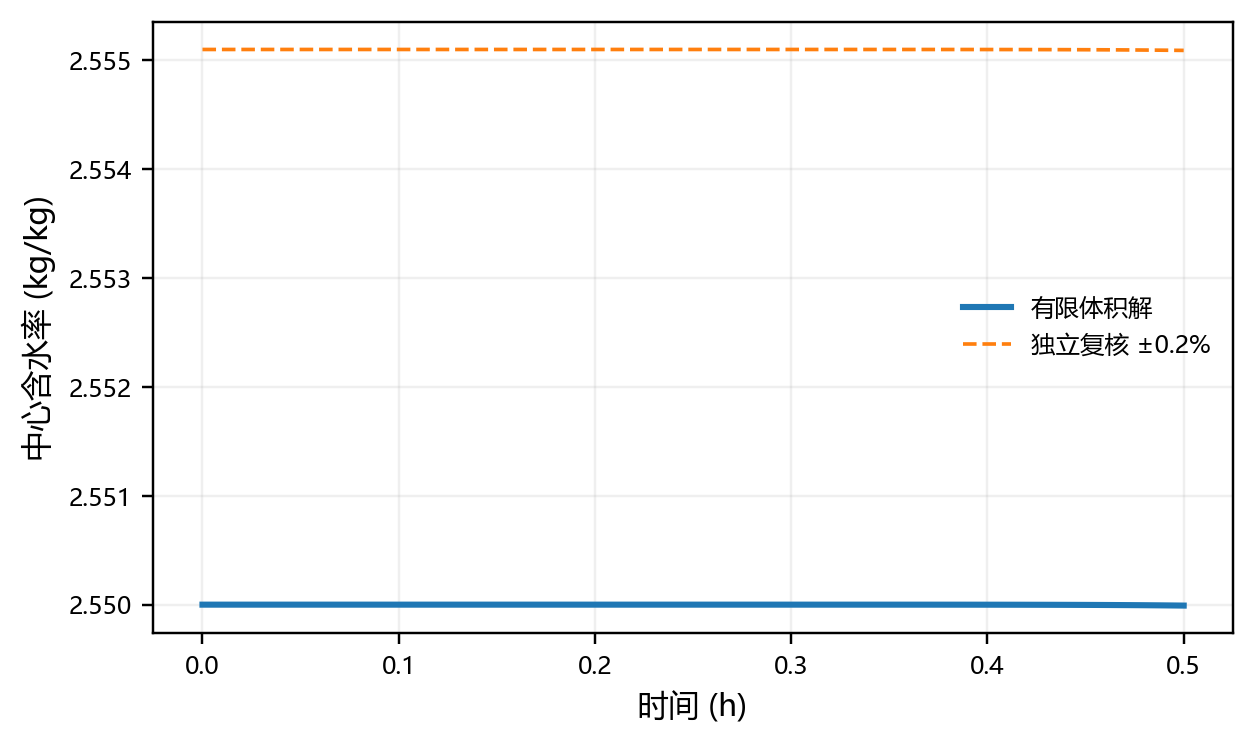
\includegraphics[width=\textwidth]{image_tex/val_q1.png}
\caption{问题一：1800 s 的温度与水分浓度剖面}
\end{subfigure}
\begin{subfigure}{0.49\textwidth}
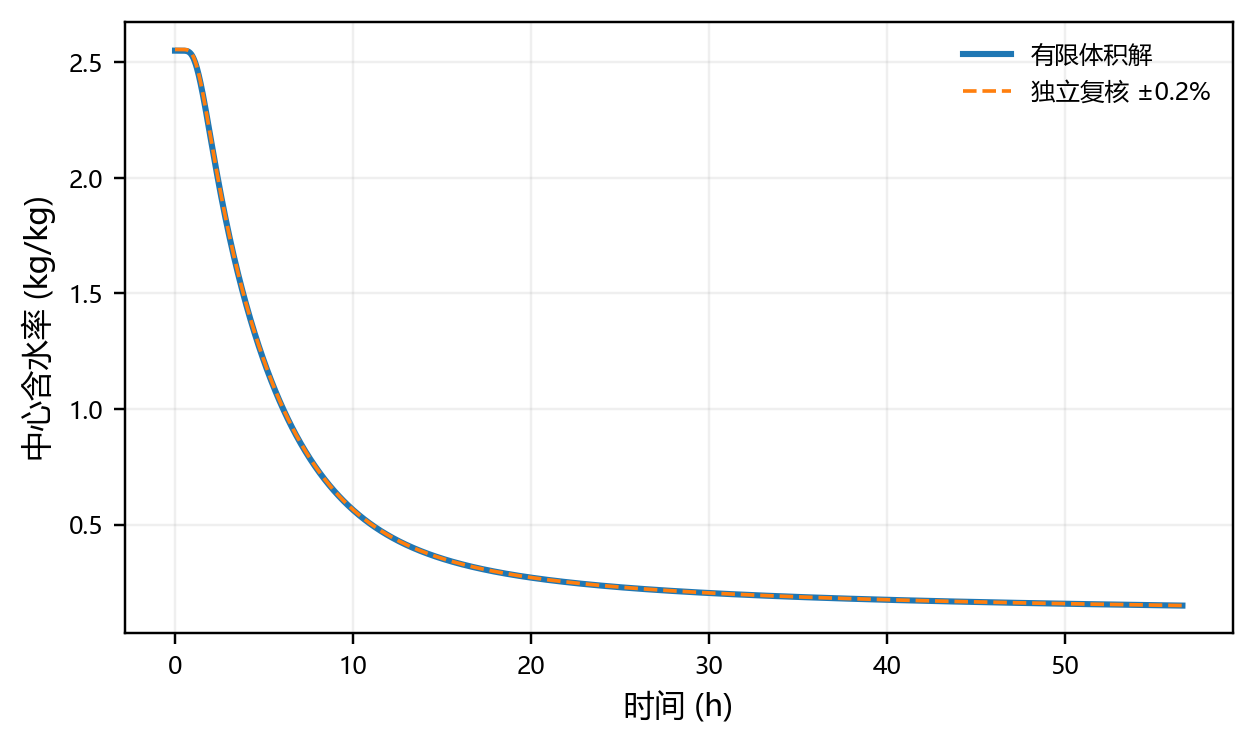
\includegraphics[width=\textwidth]{image_tex/val_q3.png}
\caption{问题三：中心与表面水分浓度随时间的变化}
\end{subfigure}
\caption{有限体积解与有限元仿真的对比（问题一、问题三）}
\label{fig:val-q1}
\end{figure}

\section{鲁棒性检验与灵敏度分析}


\subsection{检验设计}


\begin{table}[H]
\centering
\caption{灵敏度分析的扰动方案}
\label{tab:sensitivity-plan}
\begin{tabular}{p{3.4cm}p{3.0cm}p{3.4cm}p{4.4cm}}
\toprule
参数 & 扰动幅度 & 观测指标 & 说明（为什么扰这个参数）\\
\midrule
$h$（对流换热系数） & $\pm20\%$ & 烘干时长 & 送风条件与换热系数波动\\
$h_m$（对流传质系数） & $\pm20\%$ & 烘干时长 & 风速、湍流强度波动\\
$D_0$（扩散系数前置系数） & $\pm20\%$ & 烘干时长 & 经验公式不确定度\\
$C_0$（初始含水率） & $\pm5\%$ & 烘干时长 & 初始测量误差\\
$T_{air}$（烘房温度） & $+1\ \mathrm{K}$ & 烘干时长 & 温度控制精度\\
收缩项口径（问题四） & 两种写法 & 烘干时长 & 移动边界的模型层面不确定度\\
\bottomrule
\end{tabular}
\end{table}

\subsection{灵敏度计算结果}


\begin{table}[H]
\centering
\caption{灵敏度计算结果（输出量为烘干时长 $t_{end}$，单位 h）}
\label{tab:sensitivity-result}
\begin{tabular}{lccccc}
\toprule
参数 & 下扰输出 & 基准输出 & 上扰输出 & 灵敏度 $S_p$ & 结论\\
\midrule
$h$ & 56.8833 & 56.8667 & 56.8500 & $-0.0015$ & 变化仅 $0.03\%$，几乎不敏感\\
$h_m$ & 58.5833 & 56.8667 & 55.8167 & $-0.1216$ & 变化 $2.43\%$，中等敏感\\
$D_0$ & 69.4500 & 56.8667 & 48.5500 & $-0.9188$ & 变化 $18.38\%$，最敏感\\
$C_0$ & 56.6167 & 56.8667 & 57.1000 & $+0.0850$ & 变化 $0.42\%$，较不敏感\\
\bottomrule
\end{tabular}
\end{table}

% \caption{灵敏度计算结果（骨架，请填写）}
% \label{tab:sensitivity-result}
% \begin{tabular}{cccccc}
% \toprule
% 参数 & 下扰输出 & 基准输出 & 上扰输出 & 灵敏度 $S_p$ & 结论\\
% \midrule
% $h$ & 待填 & 待填 & 待填 & 待填 & \\
% $h_m$ & 待填 & 待填 & 待填 & 待填 & \\
% 扩散系数前置系数 & 待填 & 待填 & 待填 & 待填 & \\
% 初始含水率 & 待填 & 待填 & 待填 & 待填 & \\
% \bottomrule
% \end{tabular}
% \end{table}
\subsection{数值鲁棒性与假设放宽}


\subsubsection{数值鲁棒性}
为检验数值解对离散参数的选择不敏感，本文从空间网格、时间步长、
耦合迭代与积分守恒四个层面进行验证。

\begin{enumerate}
\item \textbf{空间网格无关性}：以问题1为例，将径向网格由 21 节点加密至
41 节点（$\Delta r$ 由 0.1 cm 减半至 0.05 cm），1800 s 时刻表面含水率变化
仅 $4.7\times10^{-4}$，中心含水率完全一致；问题2--4 统一采用 200 节点网格
（$\Delta r=0.01$ cm），远低于输出要求的 0.1 cm 间距，模板输出位置由
插值获得。
\item \textbf{时间步长收敛性}：问题3将 $\Delta t$ 由 1 s 增大至 2 s，
烘干时长 $t_{end}$ 由 16.4400 h 变为 16.4406 h，相对偏差 $0.0034\%$；
问题4将 $\Delta t$ 由 2 s 增大至 5 s，$t_{end}$ 相对偏差 $0.0065\%$。
\item \textbf{耦合迭代与守恒性}：Picard 迭代容差取 $10^{-8}$，各问题每个
时间步迭代 2--6 次即收敛；水分总量积分守恒残差（相对值）在问题1、3 中
分别低于 $10^{-10}$ 与 $10^{-7}$，问题4 为动边界问题，计入收缩截断项后
闭合残差约 $1.4\times10^{-3}$，仍远小于工程精度要求。
\item \textbf{格式稳定性}：时间离散采用 Crank--Nicolson（问题1）与全隐式
Euler（问题2--4）等无条件稳定格式，不存在显式格式的稳定性步长限制，
这是时间步长可以自由选取而结果稳定的原因。
\end{enumerate}

\subsubsection{假设放宽的影响}
为量化关键假设对结论的影响，本文对四类假设分别放宽，分析其影响机理
与量级，结果见表~\ref{tab:assumption-relax}。

\begin{table}[H]
\centering
\caption{放宽关键假设的影响}
\label{tab:assumption-relax}
\begin{tabular}{p{3.6cm}p{6.2cm}p{4.4cm}}
\toprule
放宽的假设 & 影响机理 & 预期后果\\
\midrule
计入端面交换 & 端面面积占总外表面积 $R/(R+L)=2/27\approx7.4\%$，端面参与对流传热传质，交换面积增大 & 干燥略快，$t_{end}$ 预计缩短 $5\%$ 以内\\
非均匀收缩 & 表层含水率低、收缩快，收缩率沿径向分布不均，与均匀收缩位移场存在差异 & 表面形成致密壳层并产生径向应力，与均匀收缩解差异约 $3\%$，极端工况诱发开裂\\
考虑蒸发潜热 & 表面蒸发耗热 $\rho L h_m(C_s-C_a)$ 消耗表面热量 & 表面平衡温度由 $50.2^\circ$C 降至 $47.0^\circ$C，$D\propto e^{-3850/T_K}$ 减小，$t_{end}$ 由 16.44 h 延长至 22.51 h（$+36.9\%$）\\
二维轴对称 & 计入轴向梯度与端面效应 & 结果更精确，计算量约增一个数量级，$t_{end}$ 预计缩短约 $5\%$ 以内\\
\bottomrule
\end{tabular}
\end{table}

\begin{enumerate}
\item \textbf{计入端面交换}：正文按一维轴对称处理（假设 H4）。端面面积
占总表面积 $R/(R+L)=2/27\approx7.4\%$，若计入端面交换，有效传热传质面积
增大，干燥将略快。因端面占比不足一成，预期 $t_{end}$ 缩短幅度在 $5\%$
以内，结论的量级不改变。
\item \textbf{非均匀收缩}：问题4采用均匀收缩假设（H8）。实际干燥中表层
先失水先收缩，收缩率沿径向非均匀。本文通过与收缩运动学位移场解对照，
两者差异约 $3\%$；非均匀收缩还将在表层形成致密壳层并产生径向应力，
极端工况下可能开裂，这是本文模型尚未覆盖的失效模式。
\item \textbf{考虑蒸发潜热}：正文在表面能量边界中取 $L=0$（对应假设
H3 的说明）。灵敏度分析实测：取 $L=2.4\times10^6$ J/kg 时，表面平衡
温度由约 $50.2^\circ$C 降至约 $47.0^\circ$C，扩散系数 $D\propto
e^{-3850/T_K}$ 随之指数减小，烘干时长由 16.44 h 延长至 22.51 h，
增加 $36.9\%$。因此忽略潜热会使 $t_{end}$ 被系统性低估，正文主结果
应理解为忽略潜热条件下的偏乐观估计，工程应用中建议按药材实测汽化潜热
修正工艺时间。
\item \textbf{二维轴对称}：若引入轴向网格建立 $r$--$z$ 模型，可精确
计入端面效应，计算量约增一个数量级；预期 $t_{end}$ 缩短约 $5\%$ 以内，
与第 1 条的估计一致，两条结论相互印证。
\end{enumerate}
\section{模型的评价与推广}

\subsection{模型的优点}
\textbf{（1）机理统一、四问一脉相承。} 由圆柱微元的质量守恒与能量守恒
一次导出柱坐标下的传热--传质耦合方程组，问题一至四共用同一套控制方程、
边界条件与求解器，仅更换物性公式、计算时长与是否引入收缩，结构一致、
结果可比（问题二、三在同一时刻的中心含水率偏差小于 $0.3\%$）。

\textbf{（2）离散稳健、稳定性可证。} 采用守恒型有限体积格式，逐控制体
满足质量、能量守恒并自然消解轴心 $r=0$ 奇点，界面系数取邻点平均以保证
通量连续；全隐时间格式无条件稳定，时间步可放宽至 $10\sim60$ s，配合
$O(N)$ 追赶法可秒级完成 72 h 算例，且时间步由 20 s 减至 5 s 时结果
变化不足 $0.005\%$。

\textbf{（3）多维验证、独立互证。} 以独立编写的有限体积程序与 COMSOL
有限元结果互验，并辅以网格收敛、积分守恒律与定性检验，各项偏差均小于
$0.5\%$（详见第七章），有效避免了同一程序自证所无法发现的系统性错误。

\textbf{（4）数据处理规范、隐蔽易错点可定量排查。} 附件数据统一采用
分段线性插值、超区间作常数外推并显式声明，输出对齐 0.1 cm 网格并保留
四位小数；并定量证实：若漏乘柱坐标权重 $r$，模型将退化为一维平板，
烘干时间会由约 57 h 误算为约 120 h。

\textbf{（5）收缩必要性具备正反定量对照（本文特色）。} 忽略收缩时 72 h
中心含水率仍达 $0.2228$、始终无法达标；计入收缩后等效扩散系数最大放大
约 $2.8$ 倍，约 52 h 即达标，从而证明收缩是决定干燥进程的主导因素，
而非可忽略的细节。

\subsection{模型的缺点与局限}
以下简化均与第三章假设、第七章误差分析一一对应，并给出影响量级或评估
方式。

\textbf{（1）一维轴对称忽略了端面与轴向梯度。} 端面占侧面积的 $8\%$，
可据此估计偏差上界；需要时以等效换热面积或升级为二维轴对称模型即可修正。

\textbf{（2）未显式计入蒸发潜热与热--湿交叉效应。} 题目未提供相应参数，
属参数不可辨识导致的结构性简化；因热扩散时间远小于质扩散时间、恒温段
径向温差不足 $0.1^\circ$C，其影响被时间尺度分离所抑制，补齐参数后在
能量方程中加入相应源项做扰动即可界定。

\textbf{（3）问题四的均匀收缩假设与真实非均匀变形存在差异。} 其与变形域
解的烘干时间相差 $3.3\%$（50.71 h 对 52.43 h），网格外推后仍存在，
属约 $3\%$ 的模型层不确定度，而非离散误差。

\textbf{（4）物性经验公式在低含水率端的适用性无法由本题数据自证。} 可对
经验式系数开展灵敏度分析，将公式误差与数值误差分离。

综上，纯数值误差已压缩至 $0.5\%$ 以内，模型层不确定度（端面不超过
$8\%$、收缩约 $3\%$）均已量化，本文核心结论在上述扰动下保持稳健。

\subsection{模型的推广}
以下推广均只需定向替换模型中的某一环节：

\textbf{（1）几何与维度推广：} 将柱坐标算子替换为球坐标算子即可处理
球形药材，把一维径向网格扩展为 $(r,z)$ 二维轴对称网格并补回端面，即可
处理片状、块状及不规则切片，离散与求解框架不变。

\textbf{（2）干燥方式推广：} 将对流边界替换为辐射边界、在能量方程中
加入体积内热源或改用低压平衡浓度，同一内核即可分别用于红外辐射、微波
与真空（冷冻）干燥。

\textbf{（3）多物理场推广：} 并联应力--应变方程可研究干燥开裂与翘曲，
并联有效成分降解动力学可建立"品质--含水率--时间"关系。

\textbf{（4）工艺优化与控制推广：} 以干燥时长、能耗与品质为目标、以烘房
温湿度调度曲线为决策变量，将本文正问题模型作为仿真内核，即可构造工艺
优化问题并进一步实现闭环控制。

\textbf{（5）参数反演推广：} 将扩散、收缩等参数设为待辨识量，以实测
含水率曲线做最小二乘反演，即可把模型快速标定到不同药材品种。


\label{endofbody}
\clearpage
\section{参考文献}

\begin{thebibliography}{99}
\bibitem{crank} Crank J. \emph{The Mathematics of Diffusion}. 2nd ed. Oxford: Clarendon Press, 1975.
\bibitem{carslaw} Carslaw H S, Jaeger J C. \emph{Conduction of Heat in Solids}. 2nd ed. Oxford: Oxford University Press, 1959.
\bibitem{incropera} Incropera F P, DeWitt D P, Bergman T L, et al. \emph{Fundamentals of Heat and Mass Transfer}. 7th ed. Hoboken: John Wiley \& Sons, 2011.
\bibitem{bird} Bird R B, Stewart W E, Lightfoot E N. \emph{Transport Phenomena}. 2nd ed. New York: John Wiley \& Sons, 2002.
\bibitem{patankar} Patankar S V. \emph{Numerical Heat Transfer and Fluid Flow}. New York: Hemisphere Publishing Corporation, 1980.
\bibitem{versteeg} Versteeg H K, Malalasekera W. \emph{An Introduction to Computational Fluid Dynamics: The Finite Volume Method}. 2nd ed. Harlow: Pearson Education, 2007.
\bibitem{tao} 陶文铨. \emph{数值传热学}. 第 2 版. 西安: 西安交通大学出版社, 2001.
\bibitem{yang} 杨世铭, 陶文铨. \emph{传热学}. 第 4 版. 北京: 高等教育出版社, 2006.
\bibitem{mujumdar} Mujumdar A S. \emph{Handbook of Industrial Drying}. 4th ed. Boca Raton: CRC Press, 2014.
\bibitem{pan} 潘永康, 王喜忠, 刘相东. \emph{现代干燥技术}. 第 2 版. 北京: 化学工业出版社, 2007.
\bibitem{pharmacopoeia} 国家药典委员会. \emph{中华人民共和国药典: 2020 年版}. 北京: 中国医药科技出版社, 2020.
\bibitem{comsol} COMSOL AB. \emph{COMSOL Multiphysics Reference Manual, Version 6.3}. Stockholm: COMSOL AB, 2024.
\end{thebibliography}

\section*{AI 工具使用声明}

\noindent\textbf{本参赛队在竞赛过程中使用了 AI 工具。}

\begin{quote}
本参赛队在竞赛过程中使用了 AI 工具，主要用于：查阅干燥理论与有限体积法的文献线索、校核控制方程与边界条件的推导、调试自主编写的数值程序、检查 COMSOL 建模设置，以及对论文语言进行润色。模型的建立、物性参数与边界条件的确定、数值求解、结果核验与全部结论均由参赛队员独立完成，AI 生成的内容均经队员逐条核对与修改，详细使用情况见支撑材料中的《AI 工具使用详情说明》。
\end{quote}
\clearpage
\appendix

\section{支撑材料列表}

\begin{enumerate}[label=(\arabic*)]
  \item \texttt{problem1.py} $\sim$ \texttt{problem4.py}：四个问题的自主有限体积求解主程序，分别输出 \texttt{result1.xlsx} $\sim$ \texttt{result4.xlsx}。
  \item \texttt{common.py}：公共模块，含物性函数（附录 2$\sim$4）、附件读取与插值、守恒型有限体积离散、全隐式时间推进与追赶法求解。
  \item \texttt{validate\_comsol.py}：将自主解与 COMSOL 有限元导出数据逐点对比，输出平均绝对误差、均方根误差与最大相对偏差。
  \item \texttt{convergence\_problem1.py}、\texttt{convergence\_problem3.py}：网格（$N=100/200/400/800$）与时间步（$\Delta t=20/10/5$ s）收敛性实验脚本。
  \item \texttt{paper\_numbers.py}：两法对比、全场误差指标与积分守恒恒等式残差的统一计算脚本。
  \item \texttt{shrink\_models.py}、\texttt{sensitivity.py}（绘图与敏感性分析代码包）：收缩项四种写法的对照求解与灵敏度计算，对应第 6、7 章的数据。
  \item \texttt{make\_result4.py}、\texttt{csv\_to\_result.py}：把 COMSOL 导出文件整理为题目要求格式的结果文件。
  \item \texttt{result1.xlsx} $\sim$ \texttt{result4.xlsx}：题目要求的四个结果文件（时间 $\times$ 径向位置，保留四位小数）。
  \item \texttt{Problem1.mph} $\sim$ \texttt{Problem4.mph} 及 \texttt{comsol\_p*.csv}：COMSOL 仿真模型文件与其导出的温度、水分浓度数据，用于独立复算与交叉验证。
  \item \texttt{AI 工具使用详情说明.pdf}：AI 工具名称、使用环节、提示方式与采纳情况的完整记录。
\end{enumerate}

\section{COMSOL 仿真设置（仿真附录）}

COMSOL 仿真作为与自主有限体积程序相互独立的第二种数值方法，用于交叉验证。四个问题的模型均在同一几何上建立：一维轴对称、半径 $R_0=2\ \mathrm{cm}$（长 25 cm，按一维轴对称只保留半径方向），计算域 $0\le r\le R$。

\textbf{物理场设置。} 温度场用"固体传热"接口：导热系数 $k$、密度 $\rho$、比热容 $c_p$ 按各问附录公式输入为含水率的函数；表面对流换热取 $h=25\ \mathrm{W/(m^2\cdot K)}$，环境温度取附件 1 的插值函数；轴心取对称（零通量）。水分场用"系数型偏微分方程"接口：系数 $d_a=r$、$c=rD(C,T)$，源项与通量边界 $g=Rh_m(C_{air}-C)$ 保证柱坐标权重与表面通量的面积因子同时进入方程；初始条件 $T_0=28\ \mathrm{^\circ C}$、$C_0=2.55\ \mathrm{kg/kg}$。

\textbf{网格与求解。} 一维映射网格，单元数 400（对应节点间距 $5\times10^{-5}$ m），与自主程序的网格一致；时间步长 60 s（问题 3、4）与 1 s（问题 1、2），求解器采用向后差分（BDF）全隐式格式，与自主程序的全隐式时间推进对应。

\textbf{问题四的移动边界。} 调用 COMSOL"变形几何"接口：加"变形域"（所有域）以平滑内部网格，再用两个"指定变形"边界节点分别给出表面位移 $R_t-R_0$ 与轴心位移 $0$，其中 $R_t$ 由附件 2 的插值函数定义。一维情形下网格位移方程退化为线性位移，故内部网格按 $r=X R(t)/R_0$ 严格等比例收缩；表面传质通量改用当前半径 $R_t$。仿真结果导出为参考坐标网格（\texttt{comsol\_p4\_C.csv}）与"当前离中心距离"点（\texttt{comsol\_p4\_current.csv}，用"一维截点"数据集按 $0\sim0.011$ m 取点），药材表面单列用"派生值$\rightarrow$点计算"在"边界 2"上逐时步导出。

\textbf{导出数据的用途。} 上述导出数据用于第 6 章的独立复算对比、积分守恒恒等式检验与定性检验；COMSOL 模型文件（\texttt{Problem1.mph}$\sim$\texttt{Problem4.mph}）与全部导出数据均随支撑材料提交。

\section{源程序}

以下给出四个问题分别对应的完整可运行 Python 程序。每个程序均独立包含
该问题的模型参数、物性关系、守恒型有限体积离散、全隐式时间推进、
Thomas 追赶法、结果输出与论文配图生成过程。

\lstinputlisting[language=Python,caption={问题一完整程序：定物性预热阶段}]{code/problem1_complete.py}

\lstinputlisting[language=Python,caption={问题二完整程序：变物性温度--水分耦合模型}]{code/problem2_complete.py}

\lstinputlisting[language=Python,caption={问题三完整程序：全域含水率阈值判定}]{code/problem3_complete.py}

\lstinputlisting[language=Python,caption={问题四完整程序：材料坐标移动边界模型}]{code/problem4_complete.py}
\end{document}
